%% abtex2-modelo-artigo.tex, v-1.9.7 laurocesar
%% Copyright 2012-2018 by abnTeX2 group at http://www.abntex.net.br/ 
%%
%% This work may be distributed and/or modified under the
%% conditions of the LaTeX Project Public License, either version 1.3
%% of this license or (at your option) any later version.
%% The latest version of this license is in
%%   http://www.latex-project.org/lppl.txt
%% and version 1.3 or later is part of all distributions of LaTeX
%% version 2005/12/01 or later.
%%
%% This work has the LPPL maintenance status `maintained'.
%% 
%% The Current Maintainer of this work is the abnTeX2 team, led
%% by Lauro César Araujo. Further information are available on 
%% http://www.abntex.net.br/
%%
%% This work consists of the files abntex2-modelo-artigo.tex and
%% abntex2-modelo-references.bib
%%

% ------------------------------------------------------------------------
% ------------------------------------------------------------------------
% abnTeX2: Modelo de Artigo Acadêmico em conformidade com
% ABNT NBR 6022:2018: Informação e documentação - Artigo em publicação 
% periódica científica - Apresentação
% ------------------------------------------------------------------------
% ------------------------------------------------------------------------

\documentclass[
	% -- opções da classe memoir --
	article,			% indica que é um artigo acadêmico
	11pt,				% tamanho da fonte
	oneside,			% para impressão apenas no recto. Oposto a twoside
	a4paper,			% tamanho do papel. 
	% -- opções da classe abntex2 --
	%chapter=TITLE,		% títulos de capítulos convertidos em letras maiúsculas
	%section=TITLE,		% títulos de seções convertidos em letras maiúsculas
	%subsection=TITLE,	% títulos de subseções convertidos em letras maiúsculas
	%subsubsection=TITLE % títulos de subsubseções convertidos em letras maiúsculas
	% -- opções do pacote babel --
	english,			% idioma adicional para hifenização
	brazil,				% o último idioma é o principal do documento
	sumario=tradicional
	]{abntex2}


% ---
% PACOTES
% ---

% ---
% Pacotes fundamentais 
% ---
\usepackage{lmodern}			% Usa a fonte Latin Modern
\usepackage[T1]{fontenc}		% Selecao de codigos de fonte.
\usepackage[utf8]{inputenc}		% Codificacao do documento (conversão automática dos acentos)
\usepackage{indentfirst}		% Indenta o primeiro parágrafo de cada seção.
\usepackage{nomencl} 			% Lista de simbolos
\usepackage{color}				% Controle das cores
\usepackage{graphicx}			% Inclusão de gráficos
\usepackage{microtype} 			% para melhorias de justificação
\usepackage{svg}
\usepackage{subcaption}
% ---
		
% ---
% Pacotes adicionais, usados apenas no âmbito do Modelo Canônico do abnteX2
% ---
\usepackage{lipsum}				% para geração de dummy text
% ---
		
% ---
% Pacotes de citações
% ---
\usepackage[brazilian,hyperpageref]{backref}	 % Paginas com as citações na bibl
\usepackage[alf]{abntex2cite}	% Citações padrão ABNT
% ---

% ---
% Configurações do pacote backref
% Usado sem a opção hyperpageref de backref
\renewcommand{\backrefpagesname}{Citado na(s) página(s):~}
% Texto padrão antes do número das páginas
\renewcommand{\backref}{}
% Define os textos da citação
\renewcommand*{\backrefalt}[4]{
	\ifcase #1 %
		Nenhuma citação no texto.%
	\or
		Citado na página #2.%
	\else
		Citado #1 vezes nas páginas #2.%
	\fi}%
% ---

% --- Informações de dados para CAPA e FOLHA DE ROSTO ---
\titulo{Relatório - Projeto \\ Inteligência Artificial}
\tituloestrangeiro{Report - Project \\ Artificial Intelligence }

\autor{
Matheus H. Pimenta Z. \thanks{matheus.pimenta@outlook.com}}

\local{Brasil}
\data{2021}
% ---

% ---
% Configurações de aparência do PDF final

% alterando o aspecto da cor azul
\definecolor{blue}{RGB}{41,5,195}

% informações do PDF
\makeatletter
\hypersetup{
     	%pagebackref=true,
		pdftitle={\@title}, 
		pdfauthor={\@author},
    	pdfsubject={Modelo de artigo científico com abnTeX2},
	    pdfcreator={LaTeX with abnTeX2},
		pdfkeywords={abnt}{latex}{abntex}{abntex2}{atigo científico}, 
		colorlinks=true,       		% false: boxed links; true: colored links
    	linkcolor=blue,          	% color of internal links
    	citecolor=blue,        		% color of links to bibliography
    	filecolor=magenta,      		% color of file links
		urlcolor=blue,
		bookmarksdepth=4
}
\makeatother
% --- 

% ---
% compila o indice
% ---
\makeindex
% ---

% ---
% Altera as margens padrões
% ---
\setlrmarginsandblock{3cm}{3cm}{*}
\setulmarginsandblock{3cm}{3cm}{*}
\checkandfixthelayout
% ---

% --- 
% Espaçamentos entre linhas e parágrafos 
% --- 

% O tamanho do parágrafo é dado por:
\setlength{\parindent}{1.3cm}

% Controle do espaçamento entre um parágrafo e outro:
\setlength{\parskip}{0.2cm}  % tente também \onelineskip

% Espaçamento simples
\SingleSpacing


% ----
% Início do documento
% ----
\begin{document}

% Seleciona o idioma do documento (conforme pacotes do babel)
%\selectlanguage{english}
\selectlanguage{brazil}

% Retira espaço extra obsoleto entre as frases.
\frenchspacing 

% ----------------------------------------------------------
% ELEMENTOS PRÉ-TEXTUAIS
% ----------------------------------------------------------

%---
%
% Se desejar escrever o artigo em duas colunas, descomente a linha abaixo
% e a linha com o texto ``FIM DE ARTIGO EM DUAS COLUNAS''.
% \twocolumn[    		% INICIO DE ARTIGO EM DUAS COLUNAS
%
%---

% página de titulo principal (obrigatório)
\maketitle


% titulo em outro idioma (opcional)



% % resumo em português
% \begin{resumoumacoluna}
%  Conforme a ABNT NBR 6022:2018, o resumo no idioma do documento é elemento obrigatório. 
%  Constituído de uma sequência de frases concisas e objetivas e não de uma 
%  simples enumeração de tópicos, não ultrapassando 250 palavras, seguido, logo 
%  abaixo, das palavras representativas do conteúdo do trabalho, isto é, 
%  palavras-chave e/ou descritores, conforme a NBR 6028. (\ldots) As 
%  palavras-chave devem figurar logo abaixo do resumo, antecedidas da expressão 
%  Palavras-chave:, separadas entre si por ponto e finalizadas também por ponto.
%  
%  \vspace{\onelineskip}
%  
%  \noindent
%  \textbf{Palavras-chave}: latex. abntex. editoração de texto.
% \end{resumoumacoluna}


% resumo em inglês
% \renewcommand{\resumoname}{Abstract}
% \begin{resumoumacoluna}
%  \begin{otherlanguage*}{english}
%    According to ABNT NBR 6022:2018, an abstract in foreign language is optional.
% 
%    \vspace{\onelineskip}
%  
%    \noindent
%    \textbf{Keywords}: latex. abntex.
%  \end{otherlanguage*}  
% \end{resumoumacoluna}

% ]  				% FIM DE ARTIGO EM DUAS COLUNAS
% ---

% \begin{center}\smaller
% \textbf{Data de submissão e aprovação}: elemento obrigatório. Indicar dia, mês e ano
% 
% \textbf{Identificação e disponibilidade}: elemento opcional. Pode ser indicado 
% o endereço eletrônico, DOI, suportes e outras informações relativas ao acesso.
% \end{center}

% ----------------------------------------------------------
% ELEMENTOS TEXTUAIS
% ----------------------------------------------------------
\textual

% ----------------------------------------------------------
% Introdução
% ----------------------------------------------------------
\section{Dataset}

O dataset utilizado é composto por $50$ colunas que representam medidas topológicas de grafos e mais uma coluna representados os rótulos das classes. Foram consideradas $200$ observações ao todo, sendo $50$ observações para cada uma das $4$ classes de elementos considerados.

O primeiro tratamento realizado no dataset foi a verificação e remoção de colunas nulas, após a remoção das colunas nulas do dataset o tamanho final foi de $34$ colunas de características e $1$ coluna dos rótulos. Nenhuma observação foi desconsiderada.

Após a remoção, foi realizada a normalização dos dados de maneira que todas as características ocupassem o mesmo intervalo de valores, isto é, a mesma escala  $[0,1]$. A normalização realizada foi utilizando o valor máximo e mínimo de cada uma das características, como apresentado pela equação \ref{eq:minmax}:
\begin{equation}
\label{eq:minmax}
 x_{scale} = \frac{x - \min{x}}{\max{x}-\min{x}}
\end{equation}
onde $x$ é o valor da observação, $\min{x}$ e $\max{x}$ são o valor mínimo e máximo da característica observada, respectivamente.

A normalização é utilizada para homogeneizar os dados e diminuir viéses existentes na geração dos dados.

\subsection{Caracterização do Dataset}

Para as representação visual do dataset foram consideradas apenas $10$ colunas, sendo a primeira coluna de cada uma das $10$ medidas topológicas consideradas.

Optou-se considerar apenas $10$ colunas devido a limitação computacional da execução de um número maior de colunas, além da poluição visual caso sejam consideradas todas as $50$ colunas.

A representação utilizando gráficos do tipo scatter plot são apresentadas nas figuras \ref{fig:scatter_hist01}, \ref{fig:scatter_hist02}, \ref{fig:scatter_kde01} e \ref{fig:scatter_kde02}. Nas diagonais são representados histogramas das características e a distribuição de densidade, respectivamente. A distribuição de densidade das variáveis é uma maneira de visualizar o comportamento da variável contínua nas observações, o que é recomendado já que o dataset é composto por variáveis contínuas.

Além das representações e gráficos scatter plot, foram extraídas informações estatísticas do dataset em análise. Os dados são apresentados nas tabelas \ref{tab:est_ori} e \ref{tab:est_norm}.

Após a normalização, para a visualização da distribuição dos dados foi realizado um boxplot e um violin plot das dez características já utilizadas anteriormente, como apresentado nas figuras \ref{fig:boxplot} e \ref{fig:violin}. A escola do violin plot é justificada pela alta frequência de valores outliers nas amostras, como apresentado pelo boxplot, dessa maneira é possível verificar em qual intervalo está a maior concentração dos dados.

\begin{figure}[h!]
 \centering
 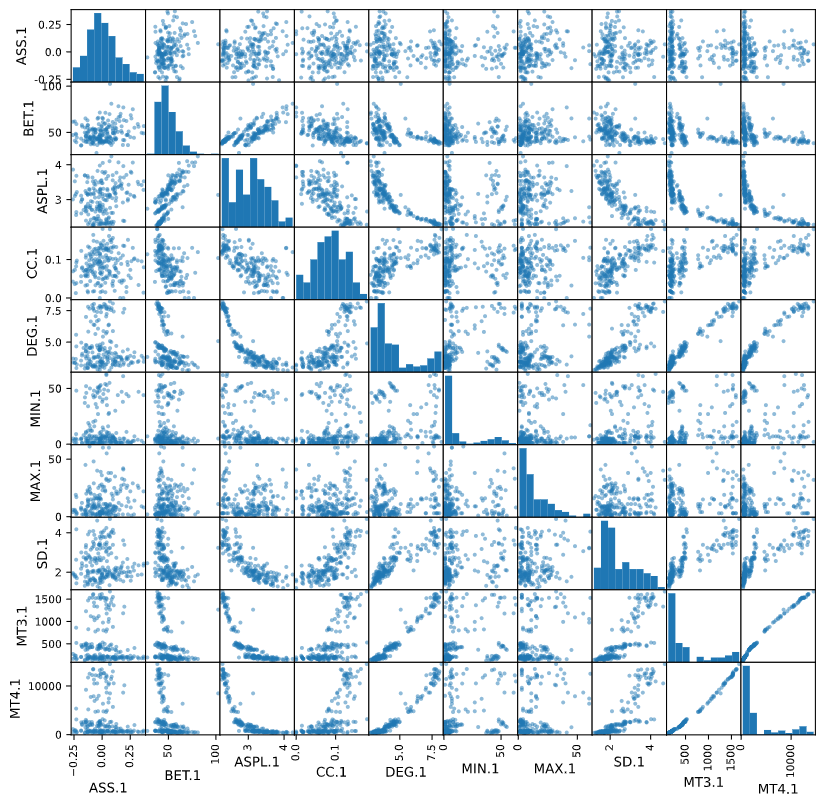
\includegraphics[scale=0.5]{fig/scatter_hist01.png}
 % scatter.png: 619x604 px, 96dpi, 16.38x15.98 cm, bb=0 0 464 453
 \caption{Representação: Scatter plot com histograma - Dataset original.}
 \label{fig:scatter_hist01}
\end{figure}

\begin{figure}[h!]
 \centering
 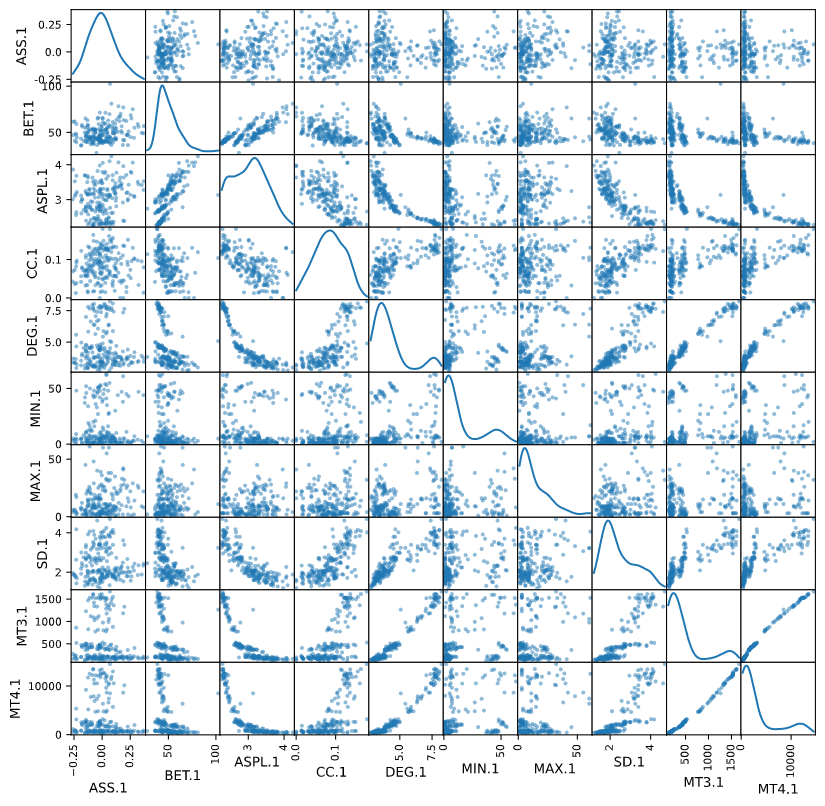
\includegraphics[scale=0.5]{fig/scatter_kde01.png}
 % scatter.png: 619x604 px, 96dpi, 16.38x15.98 cm, bb=0 0 464 453
 \caption{Representação: Scatter plot com histograma - Dataset original.}
 \label{fig:scatter_kde01}
\end{figure}


\begin{figure}[h!]
 \centering
 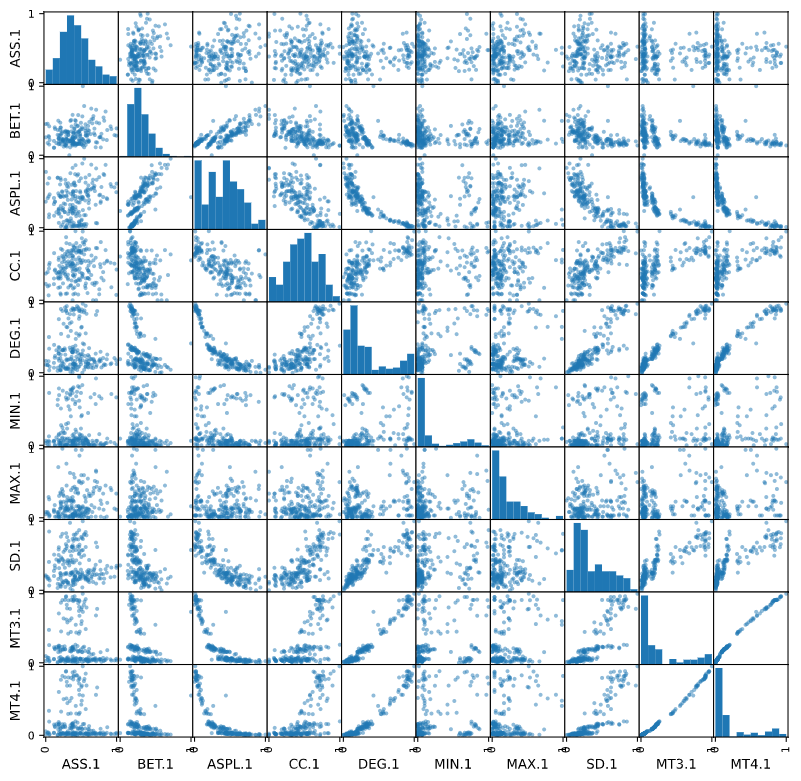
\includegraphics[scale=0.5]{fig/scatter_hist02.png}
 % scatter.png: 619x604 px, 96dpi, 16.38x15.98 cm, bb=0 0 464 453
 \caption{Representação: Scatter plot com histograma - Dataset normalizado.}
 \label{fig:scatter_hist02}
\end{figure}

\begin{figure}[h!]
 \centering
 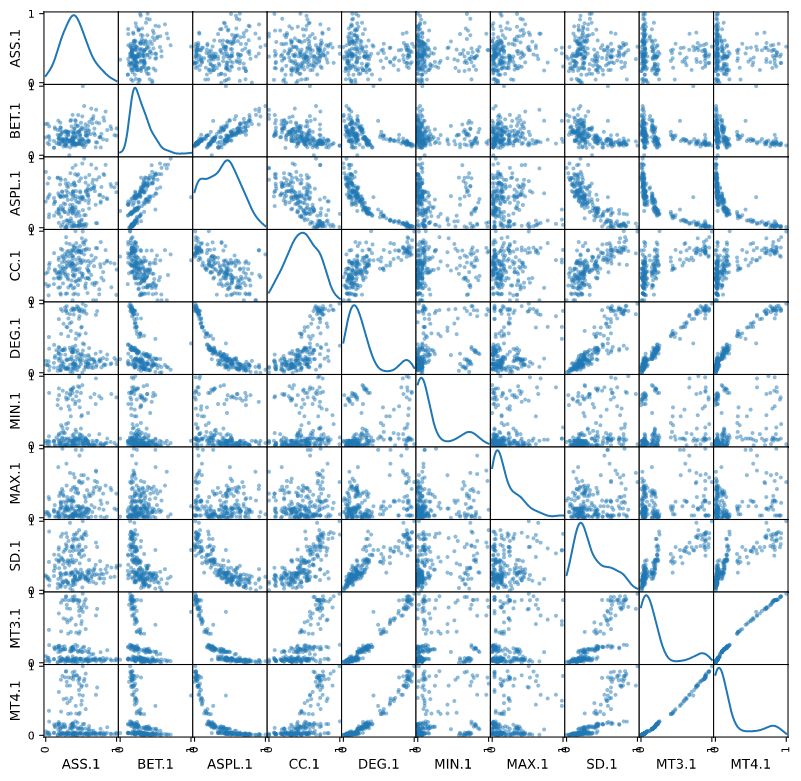
\includegraphics[scale=0.5]{fig/scatter_kde02.png}
 % scatter.png: 619x604 px, 96dpi, 16.38x15.98 cm, bb=0 0 464 453
 \caption{Representação: Scatter plot com histograma - Dataset normalizado.}
 \label{fig:scatter_kde02}
\end{figure}

\begin{table}[h!]
\small
\centering
\begin{tabular}{l|c|c|c|c|c|c|c|c|}
\cline{2-9}
                                      & count   & mean     & std      & min     & 25\%    & 50\%     & 75\%     & max       \\ \hline
\multicolumn{1}{|l|}{\textbf{ASS.1}}  & 200.000 & 0.008    & 0.131    & -0.260  & -0.081  & -0.005   & 0.086    & 0.370     \\ \hline
\multicolumn{1}{|l|}{\textbf{ASS.2}}  & 200.000 & 0.056    & 0.439    & -1.000  & -0.167  & 0.000    & 0.102    & 1.000     \\ \hline
\multicolumn{1}{|l|}{\textbf{ASS.3}}  & 200.000 & -0.008   & 0.153    & -1.000  & 0.000   & 0.000    & 0.000    & 1.000     \\ \hline
\multicolumn{1}{|l|}{\textbf{BET.1}}  & 200.000 & 49.619   & 10.103   & 27.818  & 42.495  & 47.379   & 55.014   & 102.443   \\ \hline
\multicolumn{1}{|l|}{\textbf{BET.2}}  & 200.000 & 0.195    & 0.573    & 0.000   & 0.000   & 0.017    & 0.082    & 4.000     \\ \hline
\multicolumn{1}{|l|}{\textbf{BET.3}}  & 200.000 & 0.001    & 0.008    & 0.000   & 0.000   & 0.000    & 0.000    & 0.078     \\ \hline
\multicolumn{1}{|l|}{\textbf{ASPL.1}} & 200.000 & 3.030    & 0.482    & 2.258   & 2.655   & 3.072    & 3.375    & 4.239     \\ \hline
\multicolumn{1}{|l|}{\textbf{ASPL.2}} & 200.000 & 46.516   & 17.194   & 0.000   & 43.448  & 48.695   & 58.519   & 96.856    \\ \hline
\multicolumn{1}{|l|}{\textbf{ASPL.3}} & 200.000 & 14.922   & 24.588   & 0.000   & 0.000   & 0.000    & 43.204   & 66.940    \\ \hline
\multicolumn{1}{|l|}{\textbf{ASPL.4}} & 200.000 & 1.124    & 7.939    & 0.000   & 0.000   & 0.000    & 0.000    & 62.968    \\ \hline
\multicolumn{1}{|l|}{\textbf{CC.1}}   & 200.000 & 0.085    & 0.039    & 0.000   & 0.058   & 0.086    & 0.115    & 0.180     \\ \hline
\multicolumn{1}{|l|}{\textbf{CC.2}}   & 200.000 & 0.002    & 0.016    & 0.000   & 0.000   & 0.000    & 0.000    & 0.176     \\ \hline
\multicolumn{1}{|l|}{\textbf{DEG.1}}  & 200.000 & 4.560    & 1.603    & 2.739   & 3.383   & 3.861    & 5.018    & 8.230     \\ \hline
\multicolumn{1}{|l|}{\textbf{DEG.2}}  & 200.000 & 0.486    & 0.373    & 0.000   & 0.218   & 0.400    & 0.693    & 1.651     \\ \hline
\multicolumn{1}{|l|}{\textbf{DEG.3}}  & 200.000 & 0.047    & 0.090    & 0.000   & 0.000   & 0.000    & 0.097    & 0.408     \\ \hline
\multicolumn{1}{|l|}{\textbf{DEG.4}}  & 200.000 & 0.004    & 0.026    & 0.000   & 0.000   & 0.000    & 0.000    & 0.258     \\ \hline
\multicolumn{1}{|l|}{\textbf{MIN.1}}  & 200.000 & 14.090   & 17.678   & 1.000   & 3.000   & 5.000    & 16.250   & 63.000    \\ \hline
\multicolumn{1}{|l|}{\textbf{MIN.2}}  & 200.000 & 1.370    & 1.261    & 0.000   & 1.000   & 1.000    & 1.000    & 12.000    \\ \hline
\multicolumn{1}{|l|}{\textbf{MIN.3}}  & 200.000 & 0.280    & 0.461    & 0.000   & 0.000   & 0.000    & 1.000    & 2.000     \\ \hline
\multicolumn{1}{|l|}{\textbf{MIN.4}}  & 200.000 & 0.020    & 0.140    & 0.000   & 0.000   & 0.000    & 0.000    & 1.000     \\ \hline
\multicolumn{1}{|l|}{\textbf{MAX.1}}  & 200.000 & 13.280   & 12.463   & 1.000   & 4.000   & 9.000    & 20.000   & 61.000    \\ \hline
\multicolumn{1}{|l|}{\textbf{MAX.2}}  & 200.000 & 14.210   & 14.217   & 0.000   & 2.000   & 10.500   & 22.000   & 64.000    \\ \hline
\multicolumn{1}{|l|}{\textbf{MAX.3}}  & 200.000 & 4.675    & 9.666    & 0.000   & 0.000   & 0.000    & 5.000    & 61.000    \\ \hline
\multicolumn{1}{|l|}{\textbf{MAX.4}}  & 200.000 & 0.315    & 2.685    & 0.000   & 0.000   & 0.000    & 0.000    & 27.000    \\ \hline
\multicolumn{1}{|l|}{\textbf{SD.1}}   & 200.000 & 2.438    & 0.815    & 1.195   & 1.797   & 2.118    & 3.012    & 4.699     \\ \hline
\multicolumn{1}{|l|}{\textbf{SD.2}}   & 200.000 & 0.969    & 0.526    & 0.000   & 0.668   & 0.977    & 1.312    & 2.627     \\ \hline
\multicolumn{1}{|l|}{\textbf{SD.3}}   & 200.000 & 0.197    & 0.341    & 0.000   & 0.000   & 0.000    & 0.535    & 1.435     \\ \hline
\multicolumn{1}{|l|}{\textbf{SD.4}}   & 200.000 & 0.016    & 0.116    & 0.000   & 0.000   & 0.000    & 0.000    & 0.991     \\ \hline
\multicolumn{1}{|l|}{\textbf{MT3.1}}  & 200.000 & 523.565  & 472.070  & 125.000 & 192.000 & 291.500  & 590.500  & 1669.000  \\ \hline
\multicolumn{1}{|l|}{\textbf{MT3.2}}  & 200.000 & 2.950    & 5.229    & 0.000   & 0.000   & 1.000    & 3.250    & 29.000    \\ \hline
\multicolumn{1}{|l|}{\textbf{MT3.3}}  & 200.000 & 0.050    & 0.313    & 0.000   & 0.000   & 0.000    & 0.000    & 3.000     \\ \hline
\multicolumn{1}{|l|}{\textbf{MT4.1}}  & 200.000 & 3318.465 & 4081.450 & 313.000 & 643.250 & 1180.500 & 3542.000 & 14500.000 \\ \hline
\multicolumn{1}{|l|}{\textbf{MT4.2}}  & 200.000 & 2.490    & 7.193    & 0.000   & 0.000   & 0.000    & 1.000    & 53.000    \\ \hline
\multicolumn{1}{|l|}{\textbf{MT4.3}}  & 200.000 & 0.015    & 0.122    & 0.000   & 0.000   & 0.000    & 0.000    & 1.000     \\ \hline
\end{tabular}
\caption{Medidas de posição e dispersão - Dataset original.}
\label{tab:est_ori}
\end{table}

\begin{table}[]
\centering
\begin{tabular}{l|c|c|c|c|c|c|c|c|}
\cline{2-9}
                                      & count   & mean  & std   & min   & 25\%  & 50\%  & 75\%  & max   \\ \hline
\multicolumn{1}{|l|}{\textbf{ASS.1}}  & 200.000 & 0.425 & 0.207 & 0.000 & 0.284 & 0.404 & 0.549 & 1.000 \\ \hline
\multicolumn{1}{|l|}{\textbf{ASS.2}}  & 200.000 & 0.528 & 0.219 & 0.000 & 0.417 & 0.500 & 0.551 & 1.000 \\ \hline
\multicolumn{1}{|l|}{\textbf{ASS.3}}  & 200.000 & 0.496 & 0.077 & 0.000 & 0.500 & 0.500 & 0.500 & 1.000 \\ \hline
\multicolumn{1}{|l|}{\textbf{BET.1}}  & 200.000 & 0.292 & 0.135 & 0.000 & 0.197 & 0.262 & 0.364 & 1.000 \\ \hline
\multicolumn{1}{|l|}{\textbf{BET.2}}  & 200.000 & 0.049 & 0.143 & 0.000 & 0.000 & 0.004 & 0.021 & 1.000 \\ \hline
\multicolumn{1}{|l|}{\textbf{BET.3}}  & 200.000 & 0.016 & 0.105 & 0.000 & 0.000 & 0.000 & 0.000 & 1.000 \\ \hline
\multicolumn{1}{|l|}{\textbf{ASPL.1}} & 200.000 & 0.390 & 0.243 & 0.000 & 0.200 & 0.411 & 0.564 & 1.000 \\ \hline
\multicolumn{1}{|l|}{\textbf{ASPL.2}} & 200.000 & 0.480 & 0.178 & 0.000 & 0.449 & 0.503 & 0.604 & 1.000 \\ \hline
\multicolumn{1}{|l|}{\textbf{ASPL.3}} & 200.000 & 0.223 & 0.367 & 0.000 & 0.000 & 0.000 & 0.645 & 1.000 \\ \hline
\multicolumn{1}{|l|}{\textbf{ASPL.4}} & 200.000 & 0.018 & 0.126 & 0.000 & 0.000 & 0.000 & 0.000 & 1.000 \\ \hline
\multicolumn{1}{|l|}{\textbf{CC.1}}   & 200.000 & 0.475 & 0.216 & 0.000 & 0.321 & 0.479 & 0.637 & 1.000 \\ \hline
\multicolumn{1}{|l|}{\textbf{CC.2}}   & 200.000 & 0.011 & 0.093 & 0.000 & 0.000 & 0.000 & 0.000 & 1.000 \\ \hline
\multicolumn{1}{|l|}{\textbf{DEG.1}}  & 200.000 & 0.332 & 0.292 & 0.000 & 0.117 & 0.204 & 0.415 & 1.000 \\ \hline
\multicolumn{1}{|l|}{\textbf{DEG.2}}  & 200.000 & 0.294 & 0.226 & 0.000 & 0.132 & 0.242 & 0.420 & 1.000 \\ \hline
\multicolumn{1}{|l|}{\textbf{DEG.3}}  & 200.000 & 0.116 & 0.221 & 0.000 & 0.000 & 0.000 & 0.238 & 1.000 \\ \hline
\multicolumn{1}{|l|}{\textbf{DEG.4}}  & 200.000 & 0.014 & 0.100 & 0.000 & 0.000 & 0.000 & 0.000 & 1.000 \\ \hline
\multicolumn{1}{|l|}{\textbf{MIN.1}}  & 200.000 & 0.211 & 0.285 & 0.000 & 0.032 & 0.065 & 0.246 & 1.000 \\ \hline
\multicolumn{1}{|l|}{\textbf{MIN.2}}  & 200.000 & 0.114 & 0.105 & 0.000 & 0.083 & 0.083 & 0.083 & 1.000 \\ \hline
\multicolumn{1}{|l|}{\textbf{MIN.3}}  & 200.000 & 0.140 & 0.231 & 0.000 & 0.000 & 0.000 & 0.500 & 1.000 \\ \hline
\multicolumn{1}{|l|}{\textbf{MIN.4}}  & 200.000 & 0.020 & 0.140 & 0.000 & 0.000 & 0.000 & 0.000 & 1.000 \\ \hline
\multicolumn{1}{|l|}{\textbf{MAX.1}}  & 200.000 & 0.205 & 0.208 & 0.000 & 0.050 & 0.133 & 0.317 & 1.000 \\ \hline
\multicolumn{1}{|l|}{\textbf{MAX.2}}  & 200.000 & 0.222 & 0.222 & 0.000 & 0.031 & 0.164 & 0.344 & 1.000 \\ \hline
\multicolumn{1}{|l|}{\textbf{MAX.3}}  & 200.000 & 0.077 & 0.158 & 0.000 & 0.000 & 0.000 & 0.082 & 1.000 \\ \hline
\multicolumn{1}{|l|}{\textbf{MAX.4}}  & 200.000 & 0.012 & 0.099 & 0.000 & 0.000 & 0.000 & 0.000 & 1.000 \\ \hline
\multicolumn{1}{|l|}{\textbf{SD.1}}   & 200.000 & 0.355 & 0.233 & 0.000 & 0.172 & 0.263 & 0.518 & 1.000 \\ \hline
\multicolumn{1}{|l|}{\textbf{SD.2}}   & 200.000 & 0.369 & 0.200 & 0.000 & 0.254 & 0.372 & 0.499 & 1.000 \\ \hline
\multicolumn{1}{|l|}{\textbf{SD.3}}   & 200.000 & 0.137 & 0.238 & 0.000 & 0.000 & 0.000 & 0.373 & 1.000 \\ \hline
\multicolumn{1}{|l|}{\textbf{SD.4}}   & 200.000 & 0.017 & 0.117 & 0.000 & 0.000 & 0.000 & 0.000 & 1.000 \\ \hline
\multicolumn{1}{|l|}{\textbf{MT3.1}}  & 200.000 & 0.258 & 0.306 & 0.000 & 0.043 & 0.108 & 0.301 & 1.000 \\ \hline
\multicolumn{1}{|l|}{\textbf{MT3.2}}  & 200.000 & 0.102 & 0.180 & 0.000 & 0.000 & 0.034 & 0.112 & 1.000 \\ \hline
\multicolumn{1}{|l|}{\textbf{MT3.3}}  & 200.000 & 0.017 & 0.104 & 0.000 & 0.000 & 0.000 & 0.000 & 1.000 \\ \hline
\multicolumn{1}{|l|}{\textbf{MT4.1}}  & 200.000 & 0.212 & 0.288 & 0.000 & 0.023 & 0.061 & 0.228 & 1.000 \\ \hline
\multicolumn{1}{|l|}{\textbf{MT4.2}}  & 200.000 & 0.047 & 0.136 & 0.000 & 0.000 & 0.000 & 0.019 & 1.000 \\ \hline
\multicolumn{1}{|l|}{\textbf{MT4.3}}  & 200.000 & 0.015 & 0.122 & 0.000 & 0.000 & 0.000 & 0.000 & 1.000 \\ \hline
\end{tabular}
\caption{Medidas de posição e dispersão - Dataset normalizado.}
\label{tab:est_norm}
\end{table}


\begin{figure}[h!]
 \centering
 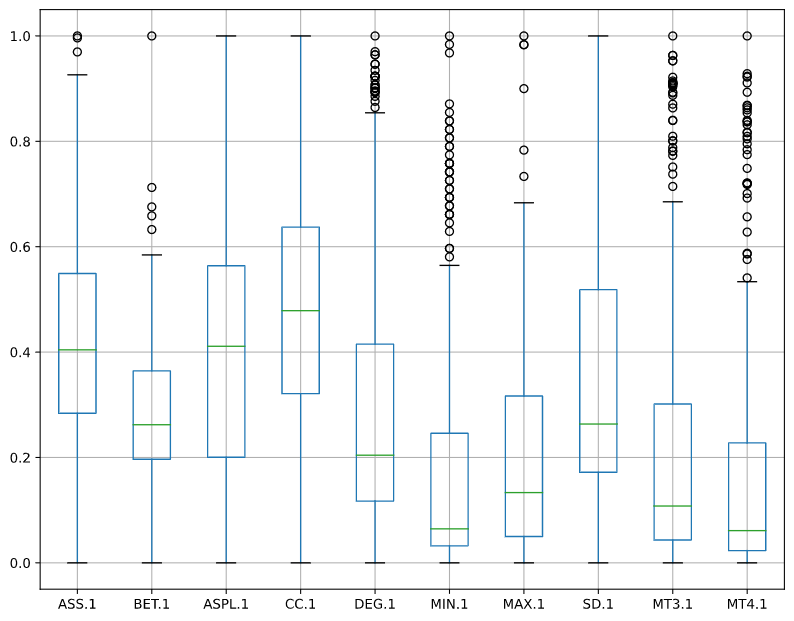
\includegraphics[scale=0.5]{fig/boxplot.png}
 % scatter.png: 619x604 px, 96dpi, 16.38x15.98 cm, bb=0 0 464 453
 \caption{Boxplot de $10$ características - Dataset normalizado.}
 \label{fig:boxplot}
\end{figure}

\begin{figure}[h!]
 \centering
 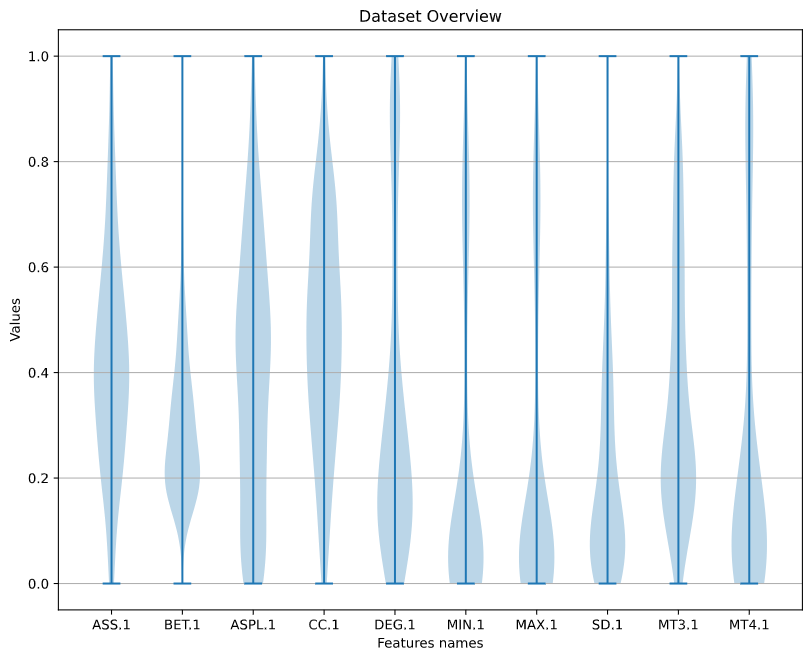
\includegraphics[scale=0.5]{fig/violin.png}
 % scatter.png: 619x604 px, 96dpi, 16.38x15.98 cm, bb=0 0 464 453
 \caption{Violin plot de $10$ características - Dataset normalizado.}
 \label{fig:violin}
\end{figure}


\section{Classificadores}

O objetivo deste trabalho é apresentar a execução de alguns classificadores, optou-se por utilizar $6$ classificadores e um dataset pequeno devido as limitações de hardware e também devido ao objetivo ante exposto. Não foram considerados classificadores do tipo \textit{ deep learning}.

O dataset foi binarizado e separado de maneira estratificada em conjuntos de treinamento e teste na seguinte proporção, $80\%$ dos dados para treinamento e $20\%$ para teste.

\subsection{k-nearest neighbors (KNN)}

O classificador k-nearest neighbors foi proposto inicialmente na década de $60$, e expandido na década de $90$ \cite{KNN}. A proposta do algoritmo é realizar a comparação da distância da $i$-ésima amostra com $k$ vizinhos mais próximos e através de votação classificar a amostra como pertencente a classe de maior votos. Os parâmetros utilizados pelo algoritmo são os seguintes:
\begin{itemize}
 \item A métrica para o cálculo da distância,
 \item O valor de $k$, isto é, quantos vizinhos serão considerados para a comparação.
\end{itemize}

As métricas mais utilizadas são a distância Euclidiana (eq. \ref{eq: dist1}), de Minkowsky (eq. \ref{eq: dist2}) e Chebyshev (eq. \ref{eq: dist3}).

\begin{eqnarray}
 \label{eq: dist1}
  d_E\left( p,q\right)&= \sqrt {\sum _{i=1}^{n}  \left( q_{i}-p_{i}\right)^2 } \\
  \label{eq: dist2}
  D_M\left( p,q\right)&= \left( \sum_{i=1}^{n} \left| p_i - q_i \right|^r \right)^{\frac{1}{r}} 
  \\
  \label{eq: dist3}
  D_C\left( p,q\right)&= \max_i(|p_i,q_i|) 
\end{eqnarray}

Já o valor de $k$ é um valor a ser definido através de um refinamento do algoritmo.

O algoritmo utilizado esta implementado no pacote \verb|sklearn.neighbors|, com a métrica padrão Euclidiana e inicialmente com o valor de $k=3$.

A acurácia e métricas obtidas para esse valor de $k$ foram as seguintes (Tabela \ref{tab:knn_01}):

\begin{table}[]
\centering
\begin{tabular}{l|c|c|c|c|}
\cline{2-5}
                                            & \textbf{precision} & \textbf{recall} & \textbf{f1-score} & \textbf{support} \\ \hline
\multicolumn{1}{|l|}{\textbf{class\_1}}     & 0.71               & 1.00            & 0.83              & 10               \\ \hline
\multicolumn{1}{|l|}{\textbf{class\_2}}     & 1.00               & 1.00            & 1.00              & 10               \\ \hline
\multicolumn{1}{|l|}{\textbf{class\_3}}     & 0.75               & 0.30            & 0.43              & 10               \\ \hline
\multicolumn{1}{|l|}{\textbf{class\_4}}     & 0.75               & 0.90            & 0.82              & 10               \\ \hline
\multicolumn{1}{|l|}{\textbf{accuracy}}     &                    &                 & 0.80              & 40               \\ \hline
\multicolumn{1}{|l|}{\textbf{macro avg}}    & 0.80               & 0.80            & 0.77              & 40               \\ \hline
\multicolumn{1}{|l|}{\textbf{weighted avg}} & 0.80               & 0.80            & 0.77              & 40               \\ \hline
\end{tabular}
\caption{Métricas - KNN - $k=3$}
\label{tab:knn_01}
\end{table}

E a seguinte matriz de confusão (Figura \ref{fig:knn_cm01}):

\begin{figure}[h!]
 \centering
 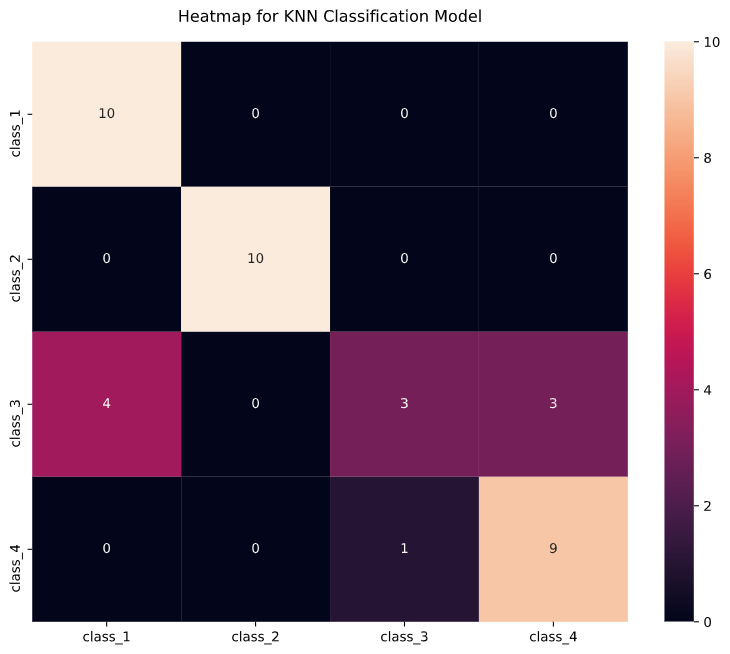
\includegraphics[scale=0.5]{fig/knn_cm01.png}
 % scatter.png: 619x604 px, 96dpi, 16.38x15.98 cm, bb=0 0 464 453
 \caption{Matriz de confusão e heatmap para o conjunto de teste - KNN - $k=3$.}
 \label{fig:knn_cm01}
\end{figure}

Com o objetivo de obter o melhor valor para $k$, foi realizada uma busca em $grid$ e para o melhor valor de $k$ em um intervalo de $[1,30]$ utilizando validação cruzada de $10-fold$. O seguinte resultado foi obtido (Figura \ref{fig:knn_grid}):

\begin{figure}[h!]
 \centering
 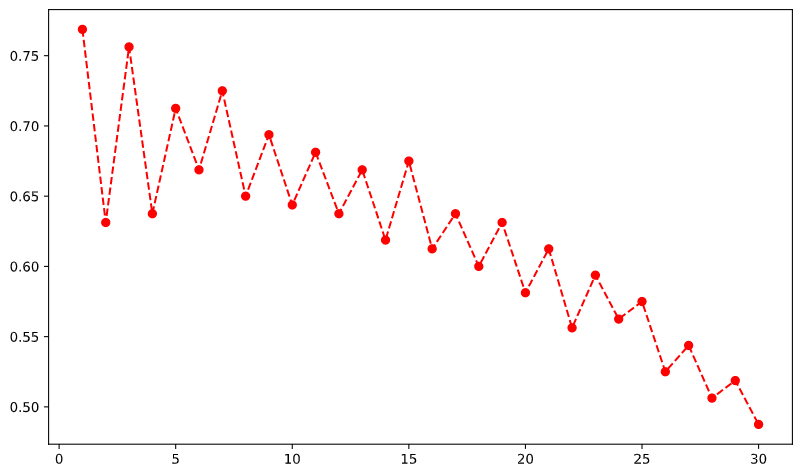
\includegraphics[scale=0.5]{fig/knn_grid.png}
 % scatter.png: 619x604 px, 96dpi, 16.38x15.98 cm, bb=0 0 464 453
 \caption{Acurácia obtida através da variação do valor de $k$.}
 \label{fig:knn_grid}
\end{figure}

Utilizando o valor da maior acurácia obtido nas validações cruzadas ($k=1$), as seguintes métricas (Tabela \ref{tab:knn_02}) e matriz de confusão (Figura \ref{fig:knn_cm02}) foram obtidas:

\begin{table}[]
\centering
\begin{tabular}{l|c|c|c|c|}
\cline{2-5}
                                            & \multicolumn{1}{l|}{\textbf{precision}} & \textbf{recall} & \textbf{f1-score} & \textbf{support} \\ \hline
\multicolumn{1}{|l|}{\textbf{class\_1}}     & 0.75                                    & 0.90            & 0.82              & 10               \\ \hline
\multicolumn{1}{|l|}{\textbf{class\_2}}     & 0.91                                    & 1.00            & 0.95              & 10               \\ \hline
\multicolumn{1}{|l|}{\textbf{class\_3}}     & 0.80                                    & 0.40            & 0.53              & 10               \\ \hline
\multicolumn{1}{|l|}{\textbf{class\_4}}     & 0.75                                    & 0.90            & 0.82              & 10               \\ \hline
\multicolumn{1}{|l|}{\textbf{accuracy}}     &                                         &                 & 0.80              & 40               \\ \hline
\multicolumn{1}{|l|}{\textbf{macro avg}}    & 0.80                                    & 0.80            & 0.78              & 40               \\ \hline
\multicolumn{1}{|l|}{\textbf{weighted avg}} & 0.80                                    & 0.80            & 0.78              & 40               \\ \hline
\end{tabular}
\caption{Métricas - KNN - $k=1$}
\label{tab:knn_02}
\end{table}

\begin{figure}[h!]
 \centering
 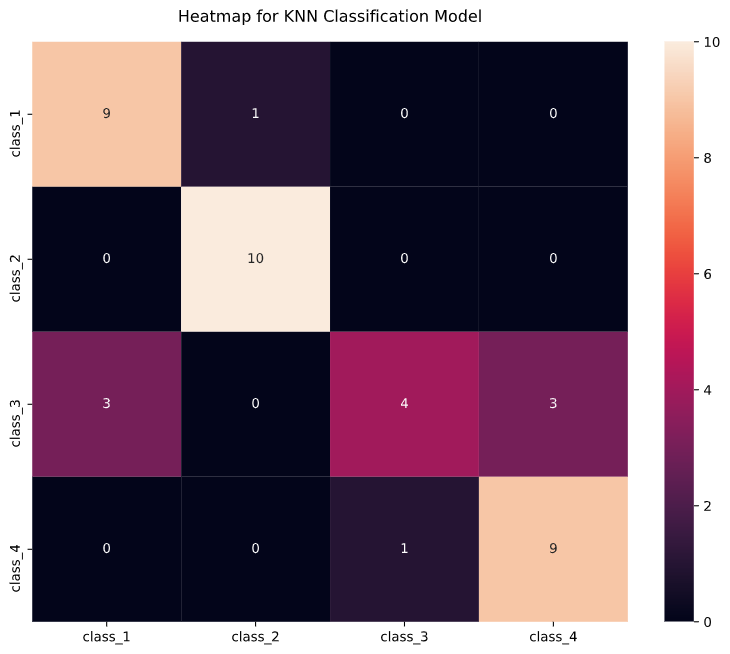
\includegraphics[scale=0.5]{fig/knn_cm02.png}
 % scatter.png: 619x604 px, 96dpi, 16.38x15.98 cm, bb=0 0 464 453
 \caption{Matriz de confusão e heatmap para o conjunto de teste - KNN - $k=1$.}
 \label{fig:knn_cm02}
\end{figure}

A análise sobre a área abaixo da curva ROC é obtida através dos seguintes gráficos para cada classe (Figura \ref{knn_roc}):

\begin{figure}
    \centering
    \begin{subfigure}[b]{0.475\textwidth}
    \centering
    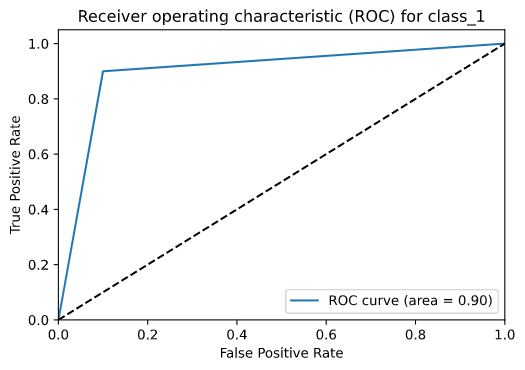
\includegraphics[scale=0.375]{fig/knn_roc1.png}
    \caption{Receiver operating characteristic (ROC) - $class_1$}
    \label{fig:knn_roc1}
    \end{subfigure}
    \hfill
    \begin{subfigure}[b]{0.475\textwidth}
    \centering
    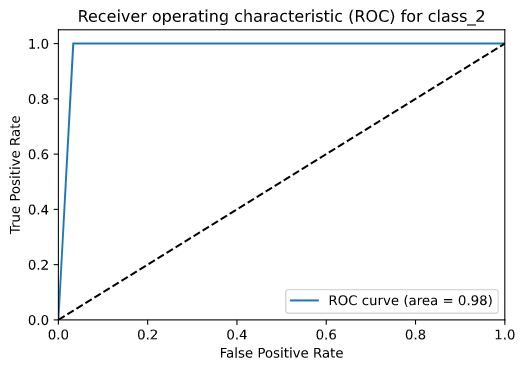
\includegraphics[scale=0.375]{fig/knn_roc2.png}
    \caption{Receiver operating characteristic (ROC) - $class_2$}
    \label{fig:knn_roc2}
    \end{subfigure}
    \vskip\baselineskip
    \begin{subfigure}[b]{0.475\textwidth}
    \centering
    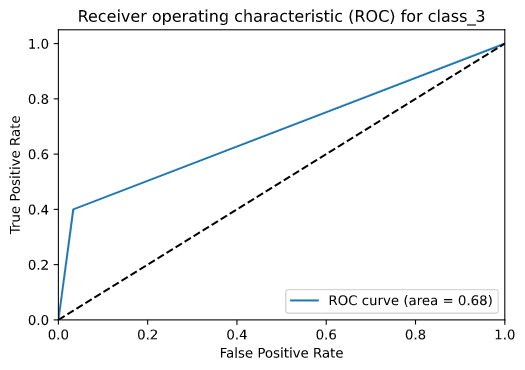
\includegraphics[scale=0.375]{fig/knn_roc3.png}
    \caption{Receiver operating characteristic (ROC) - $class_3$}
    \label{fig:knn_roc3}
    \end{subfigure}
    \hfill
    \begin{subfigure}[b]{0.475\textwidth}
    \centering
    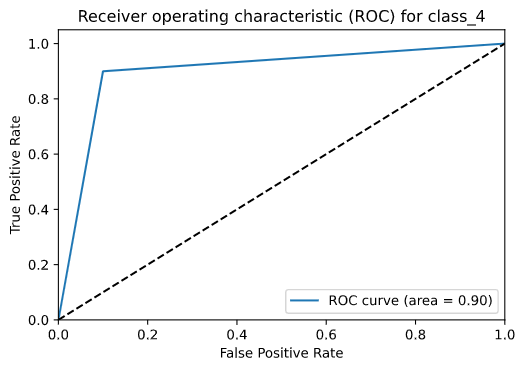
\includegraphics[scale=0.375]{fig/knn_roc4.png}
    \caption{Receiver operating characteristic (ROC) - $class_4$}
    \label{fig:knn_roc4}
    \end{subfigure}
    \caption{Receiver operating characteristic (ROC) para o classificador KNN com $k=1$.}
    \label{knn_roc}
\end{figure}

O valor do coeficiente Kappa para KNN com $k=1$ é $0.73$ com as seguintes métricas (Tabela \ref{tab:metrics_knn}).

\begin{table}[]
\centering
\begin{tabular}{|l|c|c|c|c|}
\hline
\multicolumn{1}{|c|}{\textbf{Métrica}} & \textbf{Class1} & \textbf{Class2} & \textbf{Class3} & \textbf{Class4} \\ \hline
\textbf{Sensibilidade:}                & 0.9             & 1               & 0.4             & 0.9             \\ \hline
\textbf{True Negative:}                & 0.9             & 0.96            & 0.96            & 0.9             \\ \hline
\textbf{Precisão:}                     & 0.75            & 0.9             & 0.8             & 0.75            \\ \hline
\textbf{Pred. Negativa:}               & 0.96            & 1               & 0.82            & 0.96            \\ \hline
\textbf{False Positive:}               & 0.1             & 0.03            & {]}0.03         & 0.1             \\ \hline
\textbf{False Negative:}               & 0.1             & 0               & 0.6             & 0.1             \\ \hline
\textbf{False Discovery:}              & 0.25            & 0.09            & 0.2             & 0.25            \\ \hline
\textbf{Acurácia:}                     & 0.9             & 0.97            & 0.82            & 0.9             \\ \hline
\end{tabular}
\caption{Métricas - KNN - $k=1$}
\label{tab:metrics_knn}
\end{table}

\subsection{Árvore de Decisão}

De maneira resumida, uma árvore de decisão busca relacionar os atributos (características) dos elementos (observações) com seus respectivos rótulos (classes). 

CITAR REFERÊNCIA

O algoritmo utilizado está implementado no pacote \verb|tree| da biblioteca \verb|sklearn| com o seguinte método \verb|DecisionTreeClassifier|. Os parâmetros utilizados foram todos os valores default do método.

As métricas (Tabela \ref{tab:dt_01}), matriz de confusão (Figura \ref{fig:dt_cm}) e curvas ROC (Figura \ref{dt_roc}) para cada uma das classes foram as seguintes:

\begin{table}[]
\centering
\begin{tabular}{c|c|c|c|c|}
\cline{2-5}
                                            & \textbf{precision} & \textbf{recall} & \textbf{f1-score} & \textbf{support} \\ \hline
\multicolumn{1}{|c|}{\textbf{class\_1}}     & 1.00               & 1.00            & 1.00              & 10               \\ \hline
\multicolumn{1}{|c|}{\textbf{class\_2}}     & 1.00               & 1.00            & 1.00              & 10               \\ \hline
\multicolumn{1}{|c|}{\textbf{class\_3}}     & 0.73               & 0.80            & 0.76              & 10               \\ \hline
\multicolumn{1}{|c|}{\textbf{class\_4}}     & 0.78               & 0.70            & 0.74              & 10               \\ \hline
\multicolumn{1}{|c|}{\textbf{accuracy}}     &                    &                 & 0.88              & 40               \\ \hline
\multicolumn{1}{|c|}{\textbf{macro avg}}    & 0.88               & 0.88            & 0.87              & 40               \\ \hline
\multicolumn{1}{|c|}{\textbf{weighted avg}} & 0.88               & 0.88            & 0.87              & 40               \\ \hline
\end{tabular}
\caption{Métricas - Árvore de Decisão}
\label{tab:dt_01}
\end{table}


\begin{figure}[h!]
 \centering
 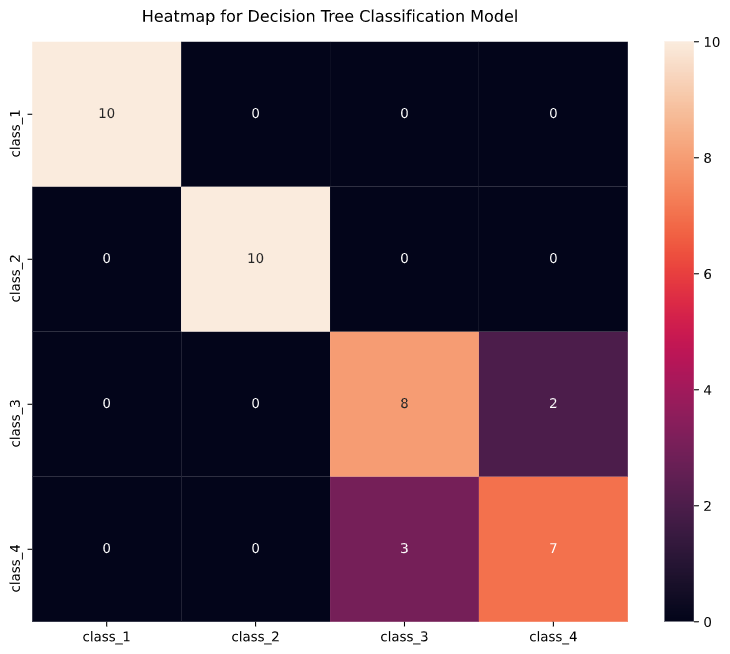
\includegraphics[scale=0.5]{fig/dt_cm.png}
 % scatter.png: 619x604 px, 96dpi, 16.38x15.98 cm, bb=0 0 464 453
 \caption{Matriz de confusão e heatmap para o conjunto de teste - Árvore de Decisão.}
 \label{fig:dt_cm}
\end{figure}

\begin{figure}
    \centering
    \begin{subfigure}[b]{0.475\textwidth}
    \centering
    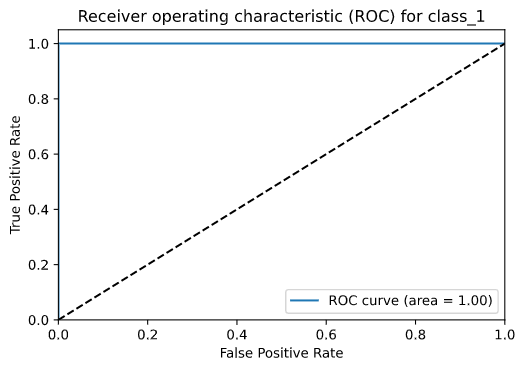
\includegraphics[scale=0.375]{fig/dt_roc1.png}
    \caption{Receiver operating characteristic (ROC) - $class_1$}
    \label{fig:dt_roc1}
    \end{subfigure}
    \hfill
    \begin{subfigure}[b]{0.475\textwidth}
    \centering
    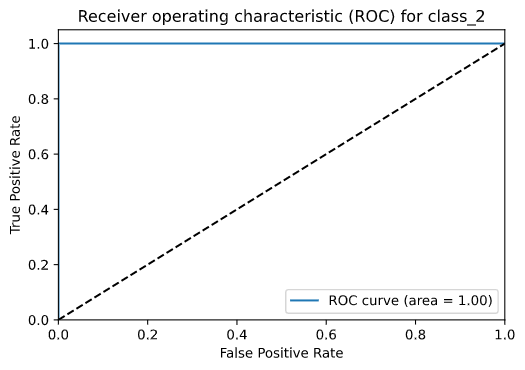
\includegraphics[scale=0.375]{fig/dt_roc2.png}
    \caption{Receiver operating characteristic (ROC) - $class_2$}
    \label{fig:dt_roc2}
    \end{subfigure}
    \vskip\baselineskip
    \begin{subfigure}[b]{0.475\textwidth}
    \centering
    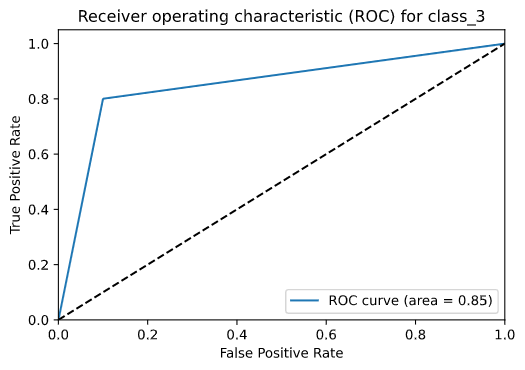
\includegraphics[scale=0.375]{fig/dt_roc3.png}
    \caption{Receiver operating characteristic (ROC) - $class_3$}
    \label{fig:dt_roc3}
    \end{subfigure}
    \hfill
    \begin{subfigure}[b]{0.475\textwidth}
    \centering
    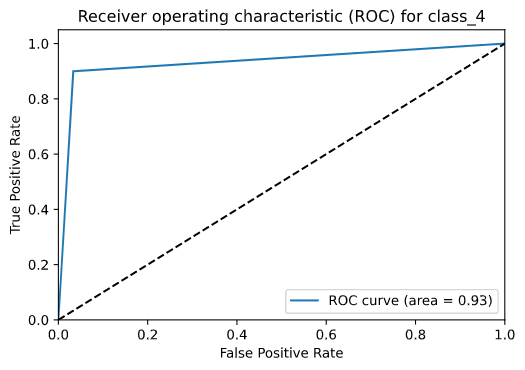
\includegraphics[scale=0.375]{fig/dt_roc4.png}
    \caption{Receiver operating characteristic (ROC) - $class_4$}
    \label{fig:dt_roc4}
    \end{subfigure}
    \caption{Receiver operating characteristic (ROC) para o classificador Árvore de Decisão.}
    \label{dt_roc}
\end{figure}

O valor do coeficiente Kappa para a Árvore de Decisão foi de $0.83$ com as seguintes métricas (Tabela \ref{tab:metrics_dt}).

\begin{table}[]
\centering
\begin{tabular}{|c|c|c|c|c|}
\hline
\textbf{Métrica}         & \textbf{Class1} & \textbf{Class2} & \textbf{Class3} & \textbf{Class4} \\ \hline
\textbf{Sensibilidade:}  & 1               & 1               & 0.8             & 0.7             \\ \hline
\textbf{True Negative:}  & 1               & 1               & 0.9             & 0.93            \\ \hline
\textbf{Precisão:}       & 1               & 1               & 0.72            & 0.77            \\ \hline
\textbf{Pred. Negativa:} & 1               & 1               & 0.93            & 0.9             \\ \hline
\textbf{False Positive:} & 0               & 0               & 0.1             & 0.06            \\ \hline
\textbf{False Negative:} & 0               & 0.              & 0.2             & 0.3             \\ \hline
\textbf{False Discovery:}    & 0               & 0               & 0.27{]}         & 0.22            \\ \hline
\textbf{Acurácia:}       & 1               & 1               & 0.87            & 0.87            \\ \hline
\end{tabular}
\caption{Métricas - Árvore de Decisão}
\label{tab:metrics_dt}
\end{table}


\subsection{Random Forest}

De maneira resumida, o algoritmo Random Forest realiza a execução de diversas árvores de decisão de maneira que  relacione os atributos (características) dos elementos (observações) com seus respectivos rótulos (classes) com uma maior assertividade. 

CITAR REFERÊNCIA

O algoritmo utilizado está implementado no pacote \verb|sklearn.ensemble| da biblioteca \verb|sklearn| com o seguinte método \verb|RandomForestClassifier|. Os parâmetros utilizados foram todos os valores default do método, isto é $100$ árvores de decisão por execução.

As métricas (Tabela \ref{tab:rf_01}), matriz de confusão (Figura \ref{fig:rf_cm}) e curvas ROC (Figura \ref{rf_roc}) para cada uma das classes foram as seguintes:

\begin{table}[]
\centering
\begin{tabular}{c|c|c|c|c|}
\cline{2-5}
                                            & \textbf{precision} & \textbf{recall} & \textbf{f1-score} & \textbf{support} \\ \hline
\multicolumn{1}{|c|}{\textbf{class\_1}}     & 0.91               & 1.00            & 0.95              & 10               \\ \hline
\multicolumn{1}{|c|}{\textbf{class\_2}}     & 1.00               & 0.90            & 0.95              & 10               \\ \hline
\multicolumn{1}{|c|}{\textbf{class\_3}}     & 0.77               & 1.00            & 0.87              & 10               \\ \hline
\multicolumn{1}{|c|}{\textbf{class\_4}}     & 1.00               & 0.70            & 0.82              & 10               \\ \hline
\multicolumn{1}{|c|}{\textbf{accuracy}}     &                    &                 & 0.90              & 40               \\ \hline
\multicolumn{1}{|c|}{\textbf{macro avg}}    & 0.92               & 0.90            & 0.90              & 40               \\ \hline
\multicolumn{1}{|c|}{\textbf{weighted avg}} & 0.92               & 0.90            & 0.90              & 40               \\ \hline
\end{tabular}
\caption{Métricas - Random Forest }
\label{tab:rf_01}
\end{table}

\begin{figure}[h!]
 \centering
 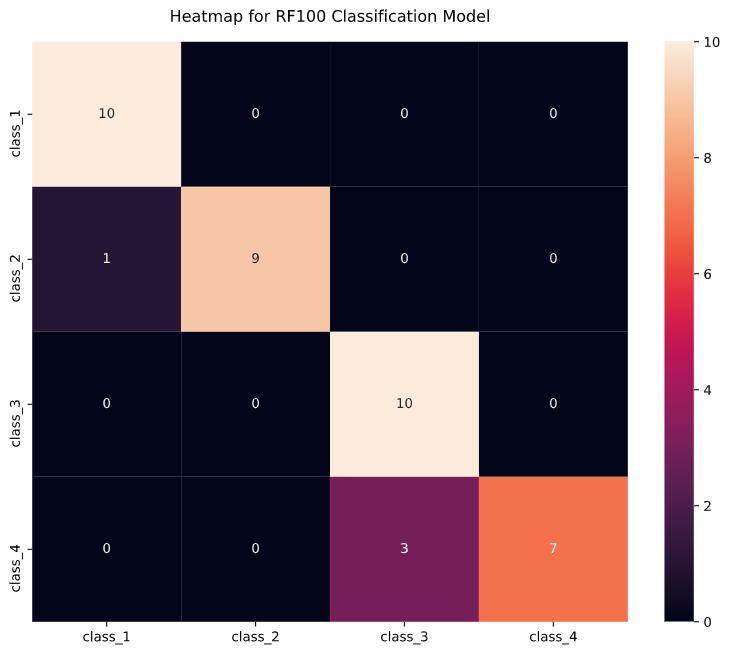
\includegraphics[scale=0.5]{fig/rf_cm.png}
 % scatter.png: 619x604 px, 96dpi, 16.38x15.98 cm, bb=0 0 464 453
 \caption{Matriz de confusão e heatmap para o conjunto de teste - Random Forest.}
 \label{fig:rf_cm}
\end{figure}


\begin{figure}
    \centering
    \begin{subfigure}[b]{0.475\textwidth}
    \centering
    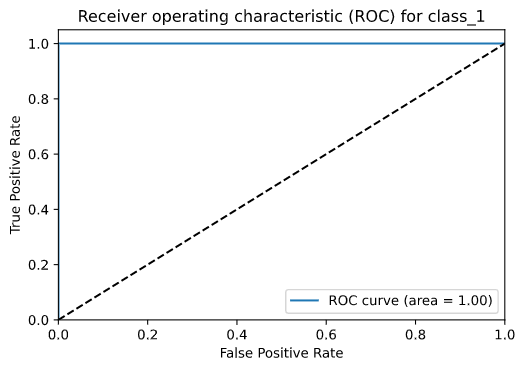
\includegraphics[scale=0.375]{fig/rf_roc1.png}
    \caption{Receiver operating characteristic (ROC) - $class_1$}
    \label{fig:rf_roc1}
    \end{subfigure}
    \hfill
    \begin{subfigure}[b]{0.475\textwidth}
    \centering
    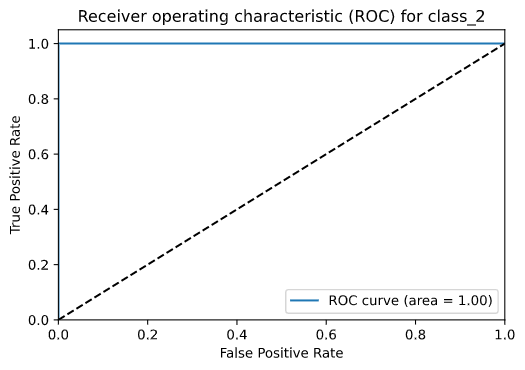
\includegraphics[scale=0.375]{fig/rf_roc2.png}
    \caption{Receiver operating characteristic (ROC) - $class_2$}
    \label{fig:rf_roc2}
    \end{subfigure}
    \vskip\baselineskip
    \begin{subfigure}[b]{0.475\textwidth}
    \centering
    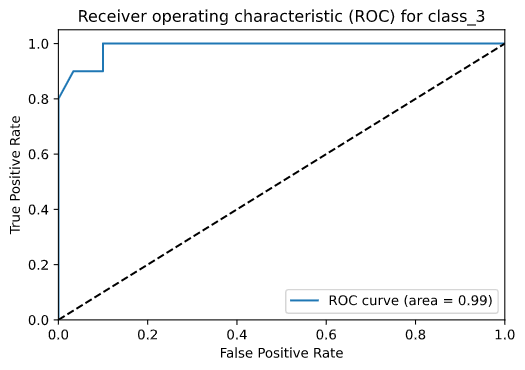
\includegraphics[scale=0.375]{fig/rf_roc3.png}
    \caption{Receiver operating characteristic (ROC) - $class_3$}
    \label{fig:rf_roc3}
    \end{subfigure}
    \hfill
    \begin{subfigure}[b]{0.475\textwidth}
    \centering
    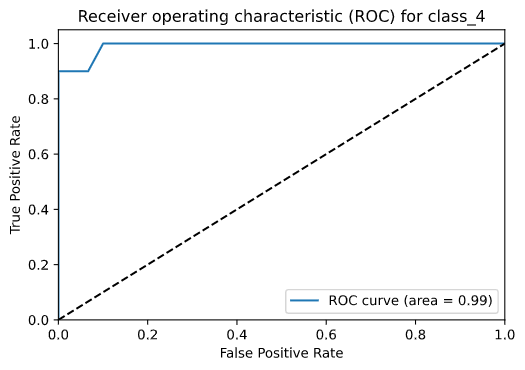
\includegraphics[scale=0.375]{fig/rf_roc4.png}
    \caption{Receiver operating characteristic (ROC) - $class_4$}
    \label{fig:rf_roc4}
    \end{subfigure}
    \caption{Receiver operating characteristic (ROC) para o classificador Random Forest.}
    \label{rf_roc}
\end{figure}

Além das análises apresentadas, foram analisados as características mais relevantes para a classificação, como apresentada na figura \ref{fig:rf_feat}.

\begin{figure}[h!]
 \centering
 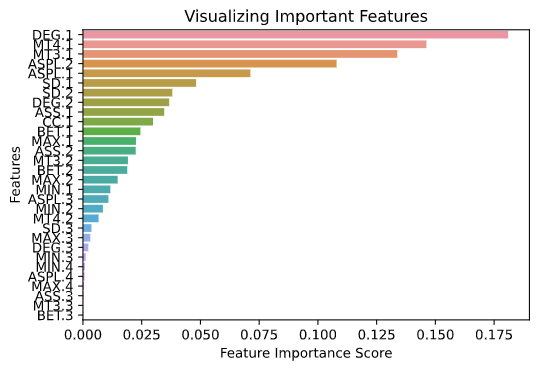
\includegraphics[scale=0.7]{fig/rf_feat.png}
 % scatter.png: 619x604 px, 96dpi, 16.38x15.98 cm, bb=0 0 464 453
 \caption{Características de maior relevância para o classificador Random Forest.}
 \label{fig:rf_feat}
\end{figure}

O valor do coeficiente Kappa para o classificador Random Forest foi de $0.86$ com as seguintes métricas (\ref{tab:metrics_rf}):

\begin{table}[]
\centering
\begin{tabular}{|c|l|l|l|l|}
\hline
\textbf{Métrica}         & \textbf{Class1} & \textbf{Class2} & \textbf{Class3} & \textbf{Class4} \\ \hline
\textbf{Sensibilidade:}  & 1               & 0.9             & 1               & 0.7             \\ \hline
\textbf{True Negative:}  & 0.96            & 1               & 0.9             & 1               \\ \hline
\textbf{Precisão:}       & 0.90            & 1               & 0.76            & 1               \\ \hline
\textbf{Pred. Negativa:} & 1               & 0.96            & 1               & 0.9             \\ \hline
\textbf{False Positive:} & 0.03            & 0               & 0.1             & 0               \\ \hline
\textbf{False Negative:} & 0               & 0.1             & 0               & 0.3             \\ \hline
\textbf{F Discovery:}    & 0.09            & 0               & 0.23            & 0               \\ \hline
\textbf{Acurácia:}       & 0.97            & 0.97            & 0.92            & 0.92            \\ \hline
\end{tabular}
\caption{Métricas - Random Forest}
\label{tab:metrics_rf}
\end{table}

\subsection{Gradient Boosting}

CITAR REFERÊNCIA

O algoritmo utilizado está implementado no pacote \verb|sklearn.ensemble| da biblioteca \verb|sklearn| com o seguinte método \verb|GradientBoostingClassifier|. 

O método possuí diversos parâmetros, como o objetivo deste relatório não é refinar métodos de machine learning optou-se por analisar somente um parâmetro do método Gradient Boosting, contudo é válido reforçar que pode-se utilizar de diversas outras abordagens para obter melhores valores nas métricas de avaliação, como por exemplo uma busca em grid de diversos parâmetros e valores.

O parâmetro analisado foi a taxa de aprendizagem do algoritmo, analisando os seguintes valores: $0.05, 0.075, 0.1, 0.25, 0.5, 0.75$ e $1$. Os demais parâmetros foram considerados os valores default. A execução com diversas taxas de aprendizagem resultou em valores de acurácia diversos 
\footnote{Os demais valores estão no arquivo grad\_boost.ipynb.}, a maior taxa de acurácia foi obtida com a taxa de $0.5$, a qual foi utilizada ao decorrer das análises. 


As métricas (Tabela \ref{tab:gb_01}), matriz de confusão (Figura \ref{fig:gb_cm}) e curvas ROC (Figura \ref{gb_roc}) para cada uma das classes foram as seguintes:

\begin{table}[]
\centering
\begin{tabular}{c|c|c|c|c|}
\cline{2-5}
                                            & \textbf{precision} & \textbf{recall} & \textbf{f1-score} & \textbf{support} \\ \hline
\multicolumn{1}{|c|}{\textbf{class\_1}}     & 1.00               & 0.80            & 0.89              & 10               \\ \hline
\multicolumn{1}{|c|}{\textbf{class\_2}}     & 1.00               & 1.00            & 1.00              & 10               \\ \hline
\multicolumn{1}{|c|}{\textbf{class\_3}}     & 0.77               & 1.00            & 0.87              & 10               \\ \hline
\multicolumn{1}{|c|}{\textbf{class\_4}}     & 1.00               & 0.90            & 0.95              & 10               \\ \hline
\multicolumn{1}{|c|}{\textbf{accuracy}}     &                    &                 & 0.93              & 40               \\ \hline
\multicolumn{1}{|c|}{\textbf{macro avg}}    & 0.94               & 0.92            & 0.93              & 40               \\ \hline
\multicolumn{1}{|c|}{\textbf{weighted avg}} & 0.94               & 0.93            & 0.93              & 40               \\ \hline
\end{tabular}
\caption{Métricas - Gradient Boosting - L.R: $0.5$}
\label{tab:gb_01}
\end{table}


\begin{figure}[h!]
 \centering
 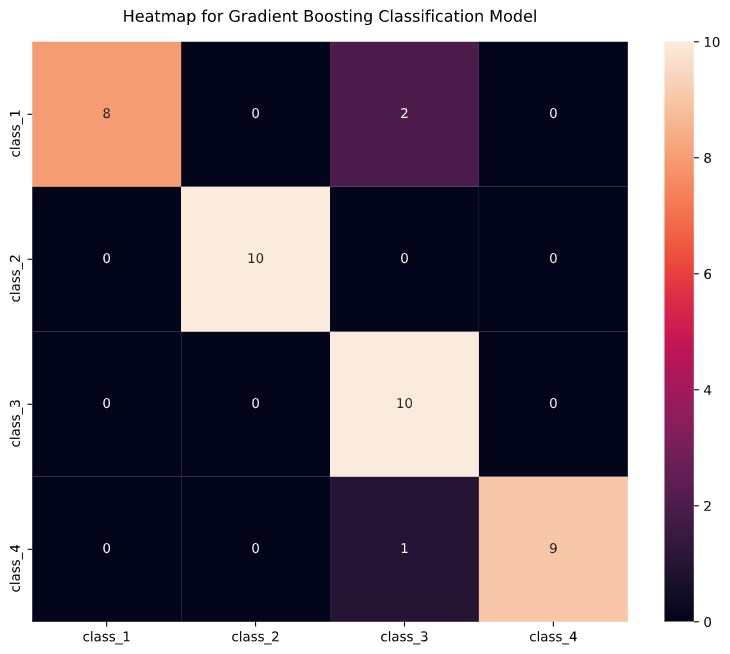
\includegraphics[scale=0.5]{fig/gb_cm.png}
 % scatter.png: 619x604 px, 96dpi, 16.38x15.98 cm, bb=0 0 464 453
 \caption{Matriz de confusão e heatmap para o conjunto de teste - Gradient Boosting L.R. :$0.5$.}
 \label{fig:gb_cm}
\end{figure}



\begin{figure}
    \centering
    \begin{subfigure}[b]{0.475\textwidth}
    \centering
    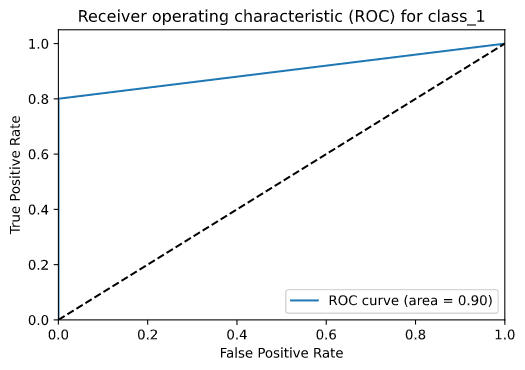
\includegraphics[scale=0.375]{fig/gb_roc1.png}
    \caption{Receiver operating characteristic (ROC) - $class_1$}
    \label{fig:gb_roc1}
    \end{subfigure}
    \hfill
    \begin{subfigure}[b]{0.475\textwidth}
    \centering
    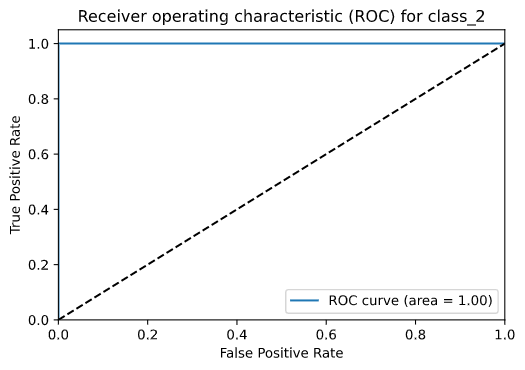
\includegraphics[scale=0.375]{fig/gb_roc2.png}
    \caption{Receiver operating characteristic (ROC) - $class_2$}
    \label{fig:gb_roc2}
    \end{subfigure}
    \vskip\baselineskip
    \begin{subfigure}[b]{0.475\textwidth}
    \centering
    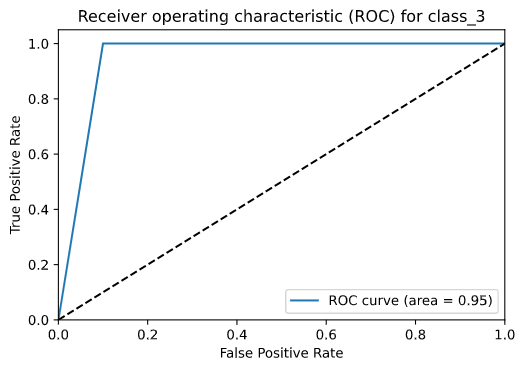
\includegraphics[scale=0.375]{fig/gb_roc3.png}
    \caption{Receiver operating characteristic (ROC) - $class_3$}
    \label{fig:gb_roc3}
    \end{subfigure}
    \hfill
    \begin{subfigure}[b]{0.475\textwidth}
    \centering
    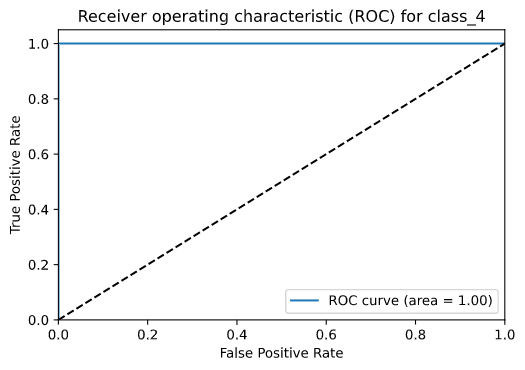
\includegraphics[scale=0.375]{fig/gb_roc4.png}
    \caption{Receiver operating characteristic (ROC) - $class_4$}
    \label{fig:gb_roc4}
    \end{subfigure}
    \caption{Receiver operating characteristic (ROC) para o classificador Grandient Boosting.}
    \label{gb_roc}
\end{figure}


O valor do coeficiente Kappa para o classificador Gradient Boosting foi de $0.9$ com as seguintes métricas (\ref{tab:metrics_gb}):

\begin{table}[]
\centering
\begin{tabular}{|c|c|c|c|c|}
\hline
\textbf{Métricas}        & \textbf{Class1} & \textbf{Class2} & \textbf{Class3} & \textbf{Class4} \\ \hline
\textbf{Sensibilidade:}  & 0.8             & 1               & 1               & 0.9             \\ \hline
\textbf{True Negative:}  & 1               & 1               & 0.9             & 1               \\ \hline
\textbf{Precisão:}       & 1               & 1               & 0.76            & 1               \\ \hline
\textbf{Pred. Negativa:} & 0.93            & 1               & 1               & 0.96            \\ \hline
\textbf{False Positive:} & 0               & 0               & 0.1             & 0               \\ \hline
\textbf{False Negative:} & 0.2             & 0               & 0               & 0.1             \\ \hline
\textbf{F Discovery:}    & 0               & 0               & 0.23            & 0               \\ \hline
\textbf{Acurácia:}       & 0.95            & 1               & 0.92            & 0.97            \\ \hline
\end{tabular}
\caption{Métricas - Gradiente Boosting - L.R.:$0.5$}
\label{tab:metrics_gb}
\end{table}

\subsection{XG Boosting}

CITAR REFERÊNCIA

O algoritmo utilizado está implementado na biblioteca \verb|xgboost| com o seguinte método \verb|XGBClassifier|. 

O método possuí diversos parâmetros, como o objetivo deste relatório não é refinar métodos de machine learning optou-se por analisar somente um parâmetro do método XG Boost, contudo é válido reforçar que pode-se utilizar de diversas outras abordagens para obter melhores valores nas métricas de avaliação, como por exemplo uma busca em grid de diversos parâmetros e valores.

O parâmetro analisado foi a taxa de aprendizagem do algoritmo, analisando os seguintes valores: $0.05, 0.075, 0.1, 0.25, 0.5, 0.75$ e $1$. Os demais parâmetros foram considerados os valores default. A execução com diversas taxas de aprendizagem resultou em valores de acurácia diversos 
\footnote{Os demais valores estão no arquivo XGBoost.ipynb.}, a maior taxa de acurácia foi obtida com a taxa de $0.075$, a qual foi utilizada ao decorrer das análises. 

As métricas (Tabela \ref{tab:xgb_01}), matriz de confusão (Figura \ref{fig:xgb_cm}) e curvas ROC (Figura \ref{xgb_roc}) para cada uma das classes foram as seguintes:

\begin{table}[]
\centering
\begin{tabular}{l|l|l|l|l|}
\cline{2-5}
                                            & \textbf{precision} & \textbf{recall} & \textbf{f1-score} & \textbf{support} \\ \hline
\multicolumn{1}{|l|}{\textbf{class\_1}}     & 0.83               & 1.00            & 0.91              & 10               \\ \hline
\multicolumn{1}{|l|}{\textbf{class\_2}}     & 1.00               & 1.00            & 1.00              & 10               \\ \hline
\multicolumn{1}{|l|}{\textbf{class\_3}}     & 0.88               & 0.70            & 0.78              & 10               \\ \hline
\multicolumn{1}{|l|}{\textbf{class\_4}}     & 0.90               & 0.90            & 0.90              & 10               \\ \hline
\multicolumn{1}{|l|}{\textbf{accuracy}}     &                    &                 & 0.90              & 40               \\ \hline
\multicolumn{1}{|l|}{\textbf{macro avg}}    & 0.90               & 0.90            & 0.90              & 40               \\ \hline
\multicolumn{1}{|l|}{\textbf{weighted avg}} & 0.90               & 0.90            & 0.90              & 40               \\ \hline
\end{tabular}
\caption{Métricas - XG Boost - L.R: $0.075$}
\label{tab:xgb_01}
\end{table}


\begin{figure}[h!]
 \centering
 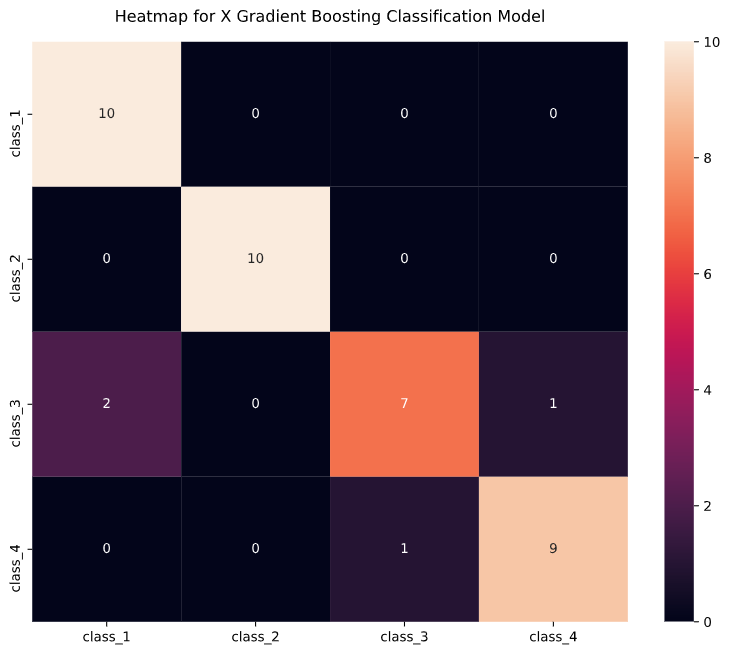
\includegraphics[scale=0.5]{fig/xgb_cm.png}
 % scatter.png: 619x604 px, 96dpi, 16.38x15.98 cm, bb=0 0 464 453
 \caption{Matriz de confusão e heatmap para o conjunto de teste - XG Boost L.R. :$0.075$.}
 \label{fig:xgb_cm}
\end{figure}


\begin{figure}
    \centering
    \begin{subfigure}[b]{0.475\textwidth}
    \centering
    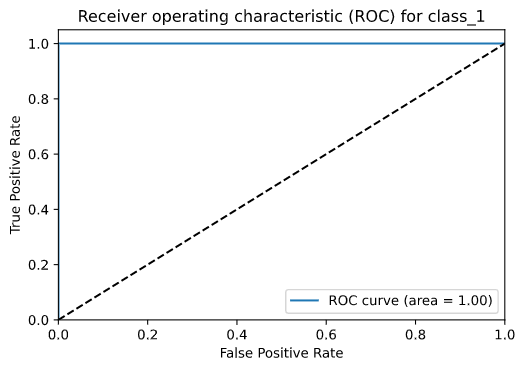
\includegraphics[scale=0.375]{fig/xgb_roc1.png}
    \caption{Receiver operating characteristic (ROC) - $class_1$}
    \label{fig:xgb_roc1}
    \end{subfigure}
    \hfill
    \begin{subfigure}[b]{0.475\textwidth}
    \centering
    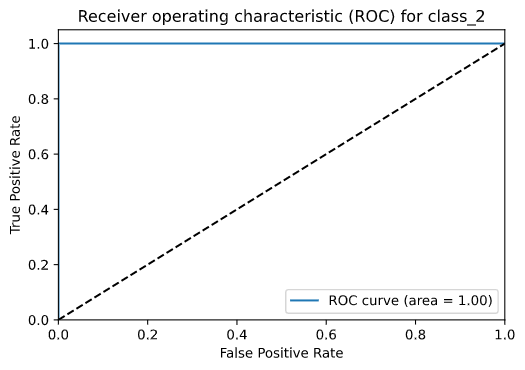
\includegraphics[scale=0.375]{fig/xgb_roc2.png}
    \caption{Receiver operating characteristic (ROC) - $class_2$}
    \label{fig:xgb_roc2}
    \end{subfigure}
    \vskip\baselineskip
    \begin{subfigure}[b]{0.475\textwidth}
    \centering
    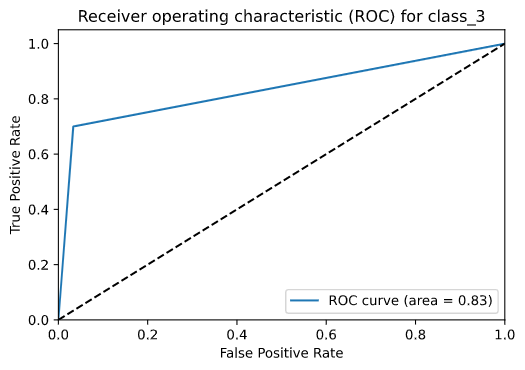
\includegraphics[scale=0.375]{fig/xgb_roc3.png}
    \caption{Receiver operating characteristic (ROC) - $class_3$}
    \label{fig:xgb_roc3}
    \end{subfigure}
    \hfill
    \begin{subfigure}[b]{0.475\textwidth}
    \centering
    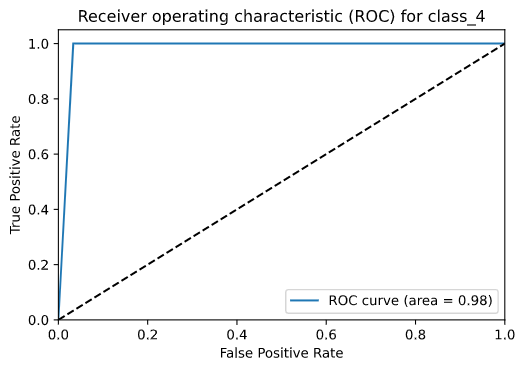
\includegraphics[scale=0.375]{fig/xgb_roc4.png}
    \caption{Receiver operating characteristic (ROC) - $class_4$}
    \label{fig:xgb_roc4}
    \end{subfigure}
    \caption{Receiver operating characteristic (ROC) para o classificador XG Boost.}
    \label{xgb_roc}
\end{figure}

O valor do coeficiente Kappa para o classificador Gradient Boosting foi de $0.86$ com as seguintes métricas (\ref{tab:metrics_xgb}):

\begin{table}[]
\centering
\begin{tabular}{|c|c|c|c|c|}
\hline
\textbf{Métrica}         & \textbf{Class1} & \textbf{Class2} & \textbf{Class3} & \textbf{Class4} \\ \hline
\textbf{Sensibilidade:}  & 1               & 1               & 0.7             & 0.9             \\ \hline
\textbf{True Negative:}  & 0.93            & 1               & 0.96            & 0.96            \\ \hline
\textbf{Precisão:}       & 0.83            & 1               & 0.87            & 0.9             \\ \hline
\textbf{Pred. Negativa:} & 1               & 1               & 0.9             & 0.96            \\ \hline
\textbf{False Positive:} & 0.06            & 0               & 0.03            & 0.03            \\ \hline
\textbf{False Negative:} & 0               & 0               & 0.3             & 0.1             \\ \hline
\textbf{F Discovery:}    & 0.16            & 0               & 0.125           & 0.1             \\ \hline
\textbf{Acurácia:}       & 0.95            & 1               & 0.9             & 0.95            \\ \hline
\end{tabular}
\caption{Métricas - XG Boost - L.R.:$0.075$}
\label{tab:metrics_xgb}
\end{table}

\subsection{Support Vector Machine (SVM)}

CITAR REFERÊNCIA

O algoritmo utilizado está implementado no pacote \verb|svm| da biblioteca \verb|sklearn| com o seguinte método \verb|SVC|. 

O método possuí diversos parâmetros, como o objetivo deste relatório não é refinar métodos de machine learning optou-se por analisar somente um parâmetro do método SVM, contudo é válido reforçar que pode-se utilizar de diversas outras abordagens para obter melhores valores nas métricas de avaliação, como por exemplo uma busca em grid de diversos parâmetros e valores.

O parâmetro analisado foi a função kernel do algoritmo, analisando o comportamento do método com seguintes kernels: \verb|'linear', 'poly', 'rbf', 'sigmoid'|. Os demais parâmetros foram considerados os valores default. A execução com diversas funções kernel resultou em valores de acurácia diversos 
\footnote{Os demais valores estão no arquivo svm.ipynb.}, a maior taxa de acurácia foi obtida com o kernel linear, o qual foi utilizado ao decorrer das análises. 

As métricas (Tabela \ref{tab:svm_01}), matriz de confusão (Figura \ref{fig:svm_cm}) e curvas ROC (Figura \ref{svm_roc}) para cada uma das classes foram as seguintes:

\begin{table}[]
\centering
\begin{tabular}{c|c|c|c|c|}
\cline{2-5}
                                            & \textbf{precision} & \textbf{recall} & \textbf{f1-score} & \textbf{support} \\ \hline
\multicolumn{1}{|c|}{\textbf{class\_1}}     & 0.59               & 1.00            & 0.74              & 10               \\ \hline
\multicolumn{1}{|c|}{\textbf{class\_2}}     & 1.00               & 1.00            & 1.00              & 10               \\ \hline
\multicolumn{1}{|c|}{\textbf{class\_3}}     & 0.67               & 0.20            & 0.31              & 10               \\ \hline
\multicolumn{1}{|c|}{\textbf{class\_4}}     & 0.90               & 0.90            & 0.90              & 10               \\ \hline
\multicolumn{1}{|c|}{\textbf{accuracy}}     &                    &                 & 0.78              & 40               \\ \hline
\multicolumn{1}{|c|}{\textbf{macro avg}}    & 0.79               & 0.78            & 0.74              & 40               \\ \hline
\multicolumn{1}{|c|}{\textbf{weighted avg}} & 0.79               & 0.78            & 0.74              & 40               \\ \hline
\end{tabular}
\caption{Métricas - SVM Linear}
\label{tab:svm_01}
\end{table}


\begin{figure}[h!]
 \centering
 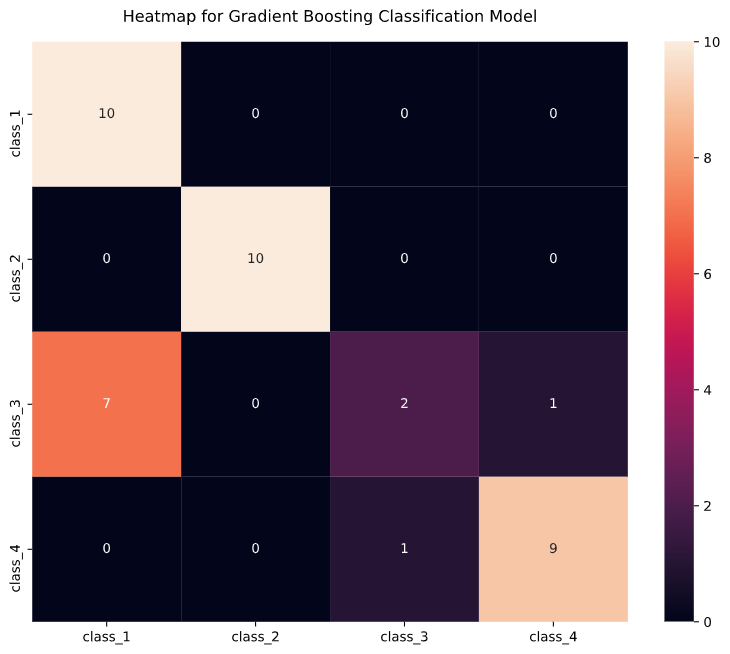
\includegraphics[scale=0.5]{fig/svm_cm.png}
 % scatter.png: 619x604 px, 96dpi, 16.38x15.98 cm, bb=0 0 464 453
 \caption{Matriz de confusão e heatmap para o conjunto de teste - SVM Linear.}
 \label{fig:svm_cm}
\end{figure}

\begin{figure}
    \centering
    \begin{subfigure}[b]{0.475\textwidth}
    \centering
    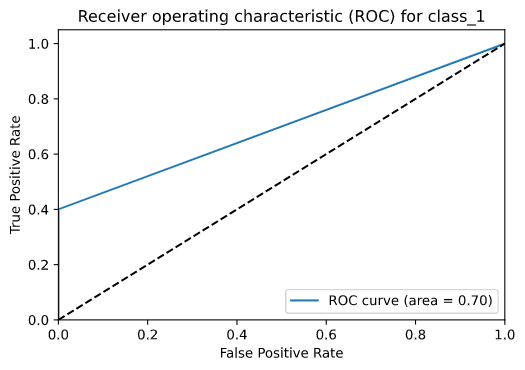
\includegraphics[scale=0.375]{fig/svm_roc1.png}
    \caption{Receiver operating characteristic (ROC) - $class_1$}
    \label{fig:svm_roc1}
    \end{subfigure}
    \hfill
    \begin{subfigure}[b]{0.475\textwidth}
    \centering
    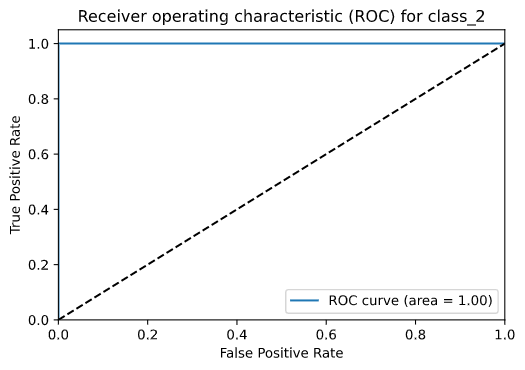
\includegraphics[scale=0.375]{fig/svm_roc2.png}
    \caption{Receiver operating characteristic (ROC) - $class_2$}
    \label{fig:svm_roc2}
    \end{subfigure}
    \vskip\baselineskip
    \begin{subfigure}[b]{0.475\textwidth}
    \centering
    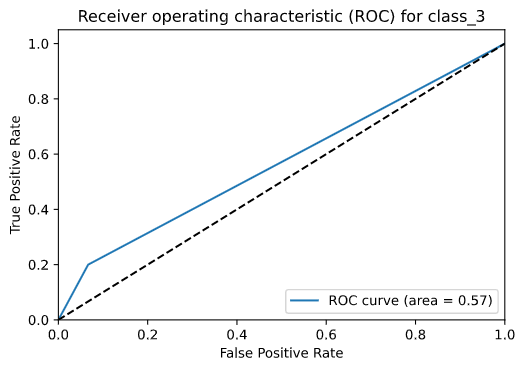
\includegraphics[scale=0.375]{fig/svm_roc3.png}
    \caption{Receiver operating characteristic (ROC) - $class_3$}
    \label{fig:svm_roc3}
    \end{subfigure}
    \hfill
    \begin{subfigure}[b]{0.475\textwidth}
    \centering
    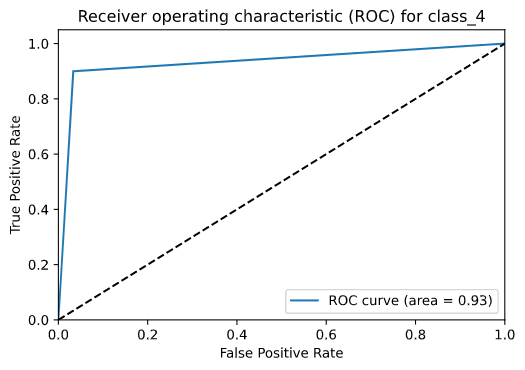
\includegraphics[scale=0.375]{fig/svm_roc4.png}
    \caption{Receiver operating characteristic (ROC) - $class_4$}
    \label{fig:svm_roc4}
    \end{subfigure}
    \caption{Receiver operating characteristic (ROC) para o classificador SVM Linear.}
    \label{svm_roc}
\end{figure}

O valor do coeficiente Kappa para o classificador Gradient Boosting foi de $0.7$ com as seguintes métricas (\ref{tab:metrics_svm}):

\begin{table}[]
\centering
\begin{tabular}{|c|c|c|c|c|}
\hline
\textbf{Métricas}        & \textbf{Class1} & \textbf{Class2} & \textbf{Class3} & \textbf{Class4} \\ \hline
\textbf{Sensibilidade:}  & 1               & 1               & 0.2             & 0.9             \\ \hline
\textbf{True Negative:}  & 0.76            & 1               & 0.96            & 0.96            \\ \hline
\textbf{Precisão:}       & 0.58            & 1               & 0.66            & 0.9             \\ \hline
\textbf{Pred. Negativa:} & 1               & 1               & 0.78            & 0.96            \\ \hline
\textbf{False Positive:} & 0.2             & 0               & 0.03            & 0.03            \\ \hline
\textbf{False Negative:} & 0               & 0               & 0.8             & 0.1             \\ \hline
\textbf{F Discovery:}    & 0.41            & 0               & 0.33            & 0.1             \\ \hline
\textbf{Acurácia:}       & 0.82            & 1               & 0.77            & 0.95            \\ \hline
\end{tabular}
\caption{Métricas - SVM Linear}
\label{tab:metrics_svm}
\end{table}



\section{Conclusão}

Realizando ROC curva para todos os métodos (Figura \ref{roc}):

\begin{figure}
    \centering
    \begin{subfigure}[b]{0.475\textwidth}
    \centering
    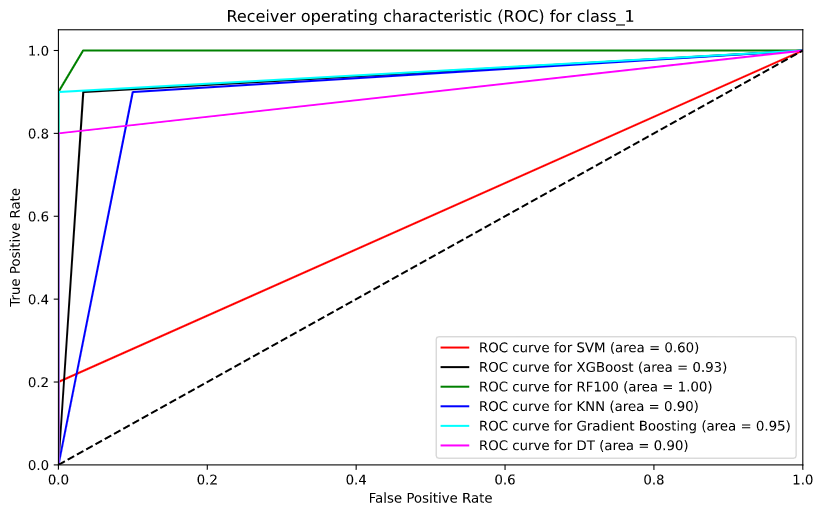
\includegraphics[scale=0.25]{fig/roc1.png}
    \caption{Receiver operating characteristic (ROC) - $class_1$}
    \label{fig:roc1}
    \end{subfigure}
    \hfill
    \begin{subfigure}[b]{0.475\textwidth}
    \centering
    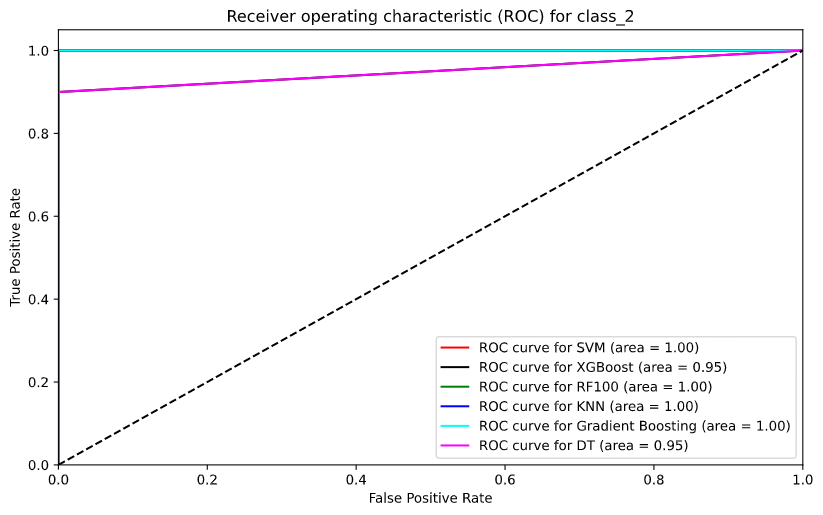
\includegraphics[scale=0.25]{fig/roc2.png}
    \caption{Receiver operating characteristic (ROC) - $class_2$}
    \label{fig:roc2}
    \end{subfigure}
    \vskip\baselineskip
    \begin{subfigure}[b]{0.475\textwidth}
    \centering
    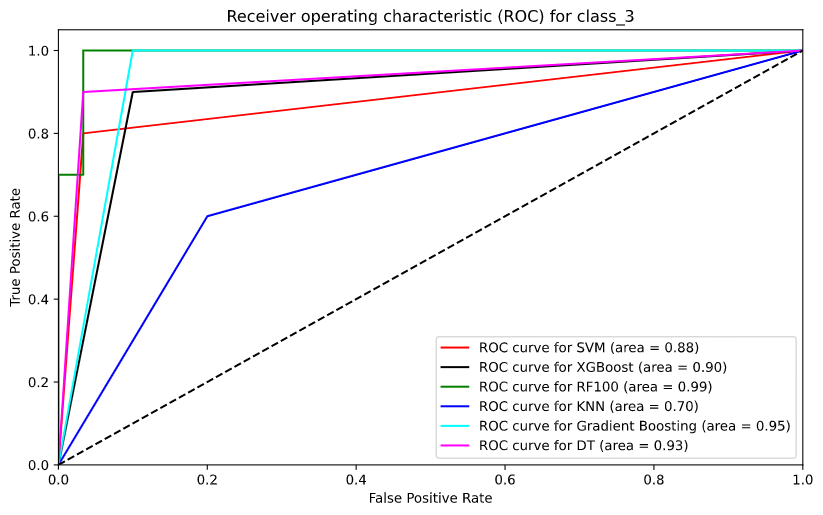
\includegraphics[scale=0.25]{fig/roc3.png}
    \caption{Receiver operating characteristic (ROC) - $class_3$}
    \label{fig:roc3}
    \end{subfigure}
    \hfill
    \begin{subfigure}[b]{0.475\textwidth}
    \centering
    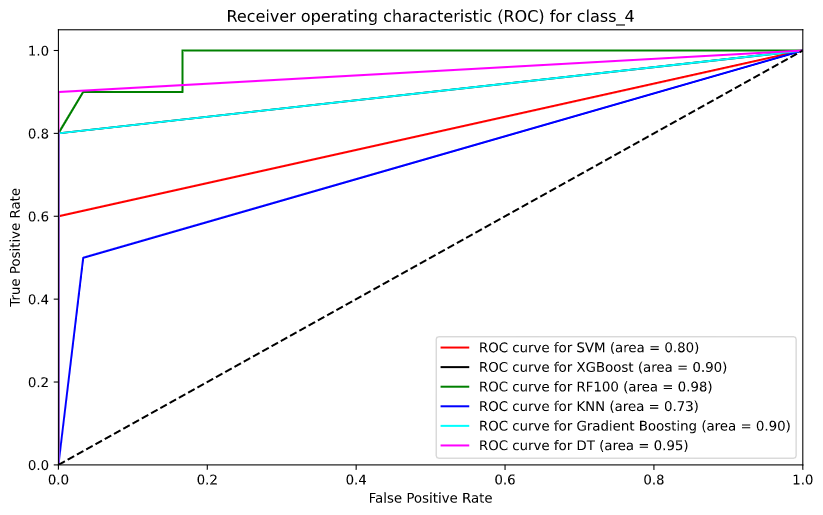
\includegraphics[scale=0.25]{fig/roc4.png}
    \caption{Receiver operating characteristic (ROC) - $class_4$}
    \label{fig:roc4}
    \end{subfigure}
    \caption{Receiver operating characteristic (ROC) para os classificadores apresentados.}
    \label{roc}
\end{figure}

E o radarplot (Figura \ref{fig:radar}):

\begin{figure}[h!]
 \centering
 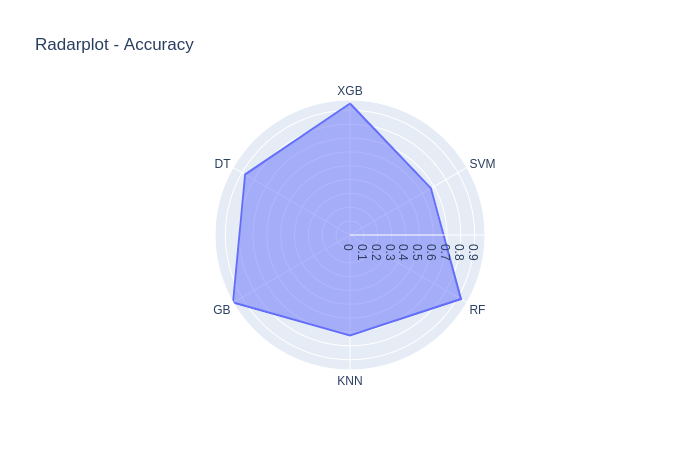
\includegraphics[scale=0.5]{fig/radarplot.png}
 % scatter.png: 619x604 px, 96dpi, 16.38x15.98 cm, bb=0 0 464 453
 \caption{Radarplot da acurácia dos métodos analisados.}
 \label{fig:radar}
\end{figure}

E barplot da acurácia dos métodos (Figura \ref{fig:barplot}):

\begin{figure}[h!]
 \centering
 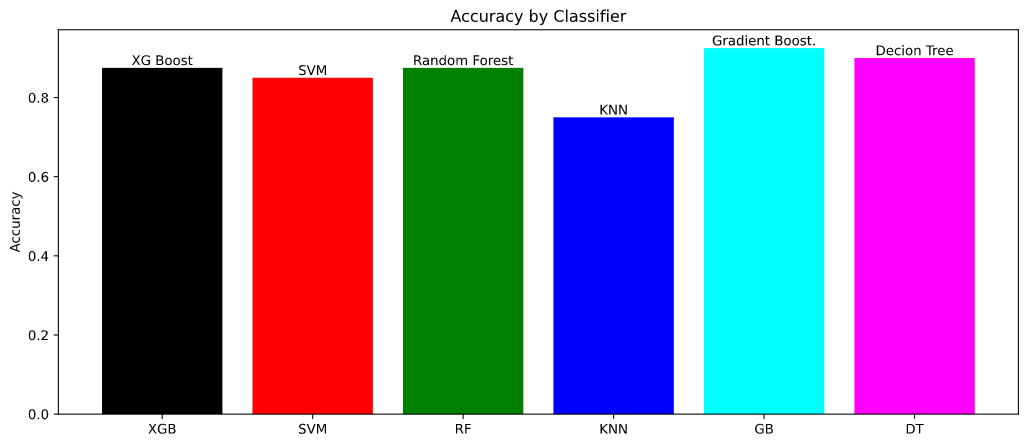
\includegraphics[scale=0.4]{fig/barplot.png}
 % scatter.png: 619x604 px, 96dpi, 16.38x15.98 cm, bb=0 0 464 453
 \caption{Barplot da acurácia dos métodos analisados.}
 \label{fig:barplot}
\end{figure}

% ----------------------------------------------------------
% ELEMENTOS PÓS-TEXTUAIS
% ----------------------------------------------------------
\postextual

% ----------------------------------------------------------
% Referências bibliográficas
% ----------------------------------------------------------
\bibliography{refs}

% ----------------------------------------------------------
% Glossário
% ----------------------------------------------------------
%
% Há diversas soluções prontas para glossário em LaTeX. 
% Consulte o manual do abnTeX2 para obter sugestões.
%
%\glossary

% ----------------------------------------------------------
% Apêndices
% ----------------------------------------------------------

% ---
% Inicia os apêndices
% ---
%\begin{apendicesenv}

% ----------------------------------------------------------
%\chapter{AA}
% ----------------------------------------------------------


%\end{apendicesenv}
% ---

% ----------------------------------------------------------
% Anexos
% ----------------------------------------------------------
%\cftinserthook{toc}{AAA}
% ---
% Inicia os anexos
% ---
%\anexos
%\begin{anexosenv}

% ---
%\chapter{Cras non urna sed feugiat cum sociis natoque penatibus et magnis dis
%parturient montes nascetur ridiculus mus}
% ---

%\lipsum[31]

%\end{anexosenv}

% ----------------------------------------------------------
% Agradecimentos
% ----------------------------------------------------------

%\section*{Agradecimentos}
%Texto sucinto aprovado pelo periódico em que será publicado. Último 
%elemento pós-textual.

\end{document}
